\documentclass[a4paper,12pt]{report}
\usepackage{a4wide}

%\documentclass[a5paper,10pt]{book}
%\usepackage[top=23mm, bottom=18mm, left=15mm, right=25mm]{geometry}
%\geometry{papersize={170mm,220mm}}


\usepackage[utf8x]{inputenc}
\usepackage[danish]{babel}

\usepackage{xr-hyper} %Externe hyper-ref
\usepackage[colorlinks=true, hyperindex=true, linkcolor=minmblaa, citecolor=minmblaa, urlcolor=minmblaa]{hyperref}
\hypersetup{colorlinks=true,filecolor=minmblaa,bookmarksnumbered=true} %Til hyperreferencer. Referencer med farver
\usepackage{needspace} % giver mulighed for at kræve at der skal være et antal tomme linier på siden før ellers indsættes et sideskift.
\usepackage{framed} %Bokse
\usepackage{wrapfig}

\usepackage{amsmath,amsfonts,amssymb,amsthm,mathtools} %Matematikpakker

\setlength{\parindent}{0mm} %Ingen Indhak i første linje i afsnit

\usepackage{color} %Farvepakke

\usepackage{array}
\usepackage{colortbl}
\usepackage{multirow} %Til at flette rækker i tabeller.

\usepackage{verbatim,mhchem}



	% DOWNLOAD FRA: http://sarovar.org/frs/?group_id=52&release_id=97
	% Læg i directory for hoved TEX fil
%\usepackage[draft]{pdfdraftcopy}
%\draftstring{Licens: Kasper Langt Mellemnavn Skårhøj}
%\draftfontsize{30}
	%\draftfontfamily{hlh}
	%\draftangle{45}
	%\definecolor{mycolor}{rgb}{.825,.855,1}
	%\draftcolor{mycolor}
	%\draftfontattrib



% = Sidehoved =
\usepackage{fancyhdr}
\pagestyle{fancy}
\renewcommand{\sectionmark}[1]{\markright{\protect\titlegraphic{dturoed}\textcolor{dtugraa}{\thesection~\MakeUppercase{#1}}}} % \thesection.\
\fancyhead{}
\fancyfoot{}
\fancyhead[R]{\titlefont\thepage}
\fancyhead[C]{}
\fancyhead[L]{\titlefont \small eNote \MakeUppercase{~\thechapter}~\hspace*{1ex}\rightmark}
\renewcommand\headrulewidth{0pt}
\fancypagestyle{plain}{\fancyfoot[C]{}}% {\titlefont\footnotesize\thepage}}
\setlength{\headheight}{15pt}


% = Længder
%\newlength{\envtblsep}\setlength{\envtblsep}{1\FrameSep}
\newlength{\obsl}\setlength{\obsl}{\textwidth-1.2cm-13.2pt}

% Includes:

% =     Fonts (select one)    =
\usepackage{mathpazo}\linespread{1.05} % Palatino needs more leading (space between lines)
\usepackage{bm} % bold math, must be loaded after the fontpackages

% % Til overskrifter
\DeclareTextFontCommand{\th}{\fontencoding{T1}\fontfamily{phv}\fontseries{b}\selectfont}
\newcommand\titlefont{\fontencoding{T1}\fontfamily{phv}\selectfont}


% =     PGF grafik      =
\usepackage{tikz}
\newcommand\titlegraphic[1]{%
\tikz[baseline] %
\draw[thick,color=#1]
(0pt  ,-0.25em) -- (0pt  ,0.85em)
(2.5pt,-0.25em) -- (2.5pt,0.85em)
(5pt  ,-0.25em) -- (5pt  ,0.85em)
(7.5pt,-0.25em) -- (7.5pt,0.85em);\hspace*{0.8ex} %
}

\newcommand\titlegraphicwide[1]{%
\tikz[baseline] %
\draw[line width=0.8mm,color=#1]
(0pt  ,-0.25em) -- (0pt  ,0.85em)
(4.5pt,-0.25em) -- (4.5pt,0.85em)
(9pt  ,-0.25em) -- (9pt  ,0.85em)
(13.5pt,-0.25em) -- (13.5pt,0.85em);\hspace*{0.8ex} %
}


% =      Title Layout      =
\usepackage{titlesec}
\makeatletter
\titleformat{\chapter}
	[display] % Shape
	{\titlefont\Huge\flushleft} % Title and label format
	{\titlefont\LARGE\bfseries \titlegraphicwide{dturoed}\textcolor{dtugraa}{\@chapapp~\thechapter}} % label
	{0.9em} % label/title separation
	{} % before code
	[] % after code
\makeatother
\titleformat{\section}
	[hang] % Shape
	{\titlefont\Large\flushleft} % Title and label format
	{\thesection} % label
	{0.9em} % label/title separation
	{} % before code
	[] % after code
\titleformat{\subsection}
	[hang] % Shape
	{\titlefont\large} % Title and label format
	{\thesubsection} % label
	{0.9em} % label/title separation
	{} % before code
	[] % after code
\titlespacing{\subsection}{0pt}{*6}{*1.5}
\titleformat{\subsubsection}
	[hang] % Shape
	{\titlefont} % Title and label format
	{\thesubsubsection} % label
	{0.9em} % label/title separation
	{} % before code
	[] % after code



% = Farver
\definecolor{dturoed}{rgb}{0.6, 0.0, 0.0}
\definecolor{dtugraa}{rgb}{0.5, 0.5, 0.5}	% Lidt mørkere. Korrekt = 0.4
\definecolor{mingroenstreg}{rgb}{0.4,0.8,0}	% Sekundærfarve 14 : 102/204/0	(Forårsgrøn) -> Eksempler
\definecolor{mingroen}{rgb}{0.32,0.64,0}		% Sekundærfarve 14, 80% mørkere (tekst)
\definecolor{minorangestreg}{rgb}{1,0.6,0}		% Sekundærfarve 1 : 255/153/0	(Orange) -> Opgaver
\definecolor{minorange}{rgb}{0.8,0.48,0}		% Sekundærfarve 1 , 80% mørkere (tekst)

\definecolor{minblaa}{rgb}{0.2,0.4,0.8}	% Sekundærfarve 13 , 51/102/204 	( Blå -> Definitioner etc)
\definecolor{minmblaa}{rgb}{0.16,0.32,0.64}	% Sekundærfarve 13 , 80% mørkere (tekst)
\definecolor{thmbackground}{rgb}{0.97,.97, 0.99}	% Farve 13 - lys baggrund

\definecolor{mingraastreg}{rgb}{.5,.5,.5}
\definecolor{hvadbackground}{rgb}{0.97,.97, 0.97}
\definecolor{sumgul}{rgb}{1,1,.8}

\definecolor{hjmopgfarve}{rgb}{.96,1,.96}


% = Counter
\newcounter{evncount}[chapter]
\setcounter{evncount}{0}
\renewcommand{\theevncount}{\thechapter.\arabic{evncount}}
\renewcommand{\theequation}{\thechapter-\arabic{equation}}


% = Eksempler = example =
\newenvironment{example}[1][]{
	\refstepcounter{evncount}
	\setlength{\obsl}{\textwidth-1.2cm-13.2pt-9pt} % fix width of the info envirnment%
	\def\FrameCommand{ 
		\textcolor{mingroenstreg}{\vrule width 4pt} 
		\hspace{5pt} 
	}%
	\MakeFramed{\advance\hsize-\width \FrameRestore}%
	\needspace{3\baselineskip}
	\titlegraphic{mingroen}
	\textcolor{mingroen}{
		\th{Eksempel \theevncount \hspace*{5mm} #1}
	} 
	\vspace*{3mm}%
	\begin{small}
	\par
}
{
	\end{small}
	\endMakeFramed
}


% = Opgaver = exercise =
\newenvironment{exercise}[1][]{
	\refstepcounter{evncount}
	\setlength{\obsl}{\textwidth-1.2cm-13.2pt-9pt}% fix width of the info envirnment%
	\def\FrameCommand{
		\textcolor{minorangestreg}{\vrule width 4pt}
		\hspace{5pt}
	}%
	\MakeFramed{\advance\hsize-\width \FrameRestore}%
	\needspace{3\baselineskip}
	\titlegraphic{minorange}
	\textcolor{minorange}{
		\th{Opgave \theevncount \hspace*{5mm} #1}
	} 
	\vspace*{3mm}%
	\begin{small}
	\par
}
{
	\end{small}
	\endMakeFramed
}


% = Bevis
\newenvironment{bevis}{
	\setlength{\obsl}{\textwidth-1.2cm-13.2pt-9pt} % fix width of the info envirnment%
	\def\FrameCommand{
		\textcolor{mingraastreg}{\vrule width 4pt} 
		\hspace{5pt}
	}%
	\MakeFramed{\advance\hsize-\width \FrameRestore}%
	\needspace{3\baselineskip}
	\titlegraphic{black}
	\textcolor{black}{
		\th{Bevis}
	}
	\vspace*{3mm}%
	\begin{small}
	\par
}
{
	\bevisslut 
	\end{small}
	\endMakeFramed
}


% = Definition =
\newenvironment{definition}[1][]{
	\vspace{4mm}
	\pagebreak[1]
	\setlength{\obsl}{\textwidth-1.2cm-2\FrameSep-13.2pt}%
	\def\FrameCommand{
		\fboxsep=\FrameSep\fcolorbox{minblaa}{thmbackground}
	}
	\begin{minipage}{\textwidth}
	\MakeFramed{\advance\hsize-\width\FrameRestore}
	\refstepcounter{evncount}
	\titlegraphic{minblaa}
	\textcolor{minmblaa}{
		\th{Definition \theevncount \hspace*{5mm} #1}
	}
	\vspace*{3mm}
	\par
}
{
	\endMakeFramed 
	\end{minipage}
	\vspace{4mm}
}


% = Theorem =
\newenvironment{theorem}[1][]{
	\vspace{4mm}
	\pagebreak[1]%
	\setlength{\obsl}{\textwidth-1.2cm-2\FrameSep-13.2pt}%
	\def\FrameCommand{
		\fboxsep=\FrameSep\fcolorbox{minblaa}{thmbackground}
	}%
	\begin{minipage}{\textwidth}
	\MakeFramed{\advance\hsize-\width\FrameRestore}%
	\refstepcounter{evncount}
	\titlegraphic{minblaa}
	\textcolor{minmblaa}{
		\th{Sætning \theevncount \hspace*{5mm} #1}
	}
	\vspace*{3mm}
	\par
}
{
	\endMakeFramed 
	\end{minipage}
	\vspace{4mm}
}


% = Lemma =
\newenvironment{lemma}[1][]{
	\vspace{4mm}
	\pagebreak[1]
	\setlength{\obsl}{\textwidth-1.2cm-2\FrameSep-13.2pt}%
	\def\FrameCommand{
		\fboxsep=\FrameSep \fcolorbox{minblaa}{thmbackground}
	}
	\begin{minipage}{\textwidth} 
	\MakeFramed{\advance\hsize-\width \FrameRestore}
	\refstepcounter{evncount}
	\titlegraphic{minblaa}
	\textcolor{minmblaa}{
		\th{Hjælpesætning \theevncount \hspace*{5mm} #1}
	}
	\vspace*{3mm}
	\par
}
{
	\endMakeFramed 
	\end{minipage}
	\vspace{4mm}
}


% = Corollary =
\newenvironment{corollary}[1][]{
	\vspace{4mm}
	\pagebreak[1]
	\setlength{\obsl}{\textwidth-1.2cm-2\FrameSep-13.2pt}%
	\def\FrameCommand{
		\fboxsep=\FrameSep \fcolorbox{minblaa}{thmbackground}
	}
	\begin{minipage}{\textwidth} 
	\MakeFramed{\advance\hsize-\width \FrameRestore}
	\refstepcounter{evncount}
	\titlegraphic{minblaa}
	\textcolor{minmblaa}{
		\th{Følgesætning \theevncount \hspace*{5mm} #1}
	}
	\vspace*{3mm}
	\par
}
{
	\endMakeFramed 
	\end{minipage}
	\vspace{4mm}
}


% = Metode = method
\newenvironment{method}[1][]{
	\vspace{4mm}
	\pagebreak[1]
	\setlength{\obsl}{\textwidth-1.2cm-2\FrameSep-13.2pt}%
	\def\FrameCommand{
		\fboxsep=\FrameSep \fcolorbox{black}{hvadbackground}
	}
	\begin{minipage}{\textwidth} 
	\MakeFramed{\advance\hsize-\width \FrameRestore}
	\refstepcounter{evncount}
	\titlegraphic{black}
	\textcolor{black}{
		\th{Metode \theevncount \hspace*{5mm} #1}
	}
	\vspace*{3mm}
	\par
}
{
	\endMakeFramed
	\end{minipage}
	\vspace{4mm}
}


% = Forklaring = explain =
\newenvironment{explain}[1][]{
	\vspace{4mm}
	\pagebreak[1]
	\setlength{\obsl}{\textwidth-1.2cm-2\FrameSep-13.2pt}%
	\def\FrameCommand{
		\fboxsep=\FrameSep \fcolorbox{black}{hvadbackground}
	}
	\MakeFramed{\advance\hsize-\width \FrameRestore}
	\refstepcounter{evncount}
	\titlegraphic{black}
	\textcolor{black}{
		\th{Forklaring \theevncount \hspace*{5mm} #1}
	}
	\vspace*{3mm}
	\par
}
{
	\endMakeFramed
	\vspace{4mm}
}


% = Bemærkning = remark =
\newenvironment{remark}[1][]{
	\vspace{4mm}
	\pagebreak[1]
	\setlength{\obsl}{\textwidth-1.2cm-2\FrameSep-13.2pt}%
	\def\FrameCommand{
		\fboxsep=\FrameSep \fcolorbox{black}{hvadbackground}
	}
	\begin{minipage}{\textwidth} 
	\MakeFramed{\advance\hsize-\width \FrameRestore}
	\refstepcounter{evncount}
	\titlegraphic{black}
	\textcolor{black}{
		\th{Bemærkning \theevncount \hspace*{5mm} #1}
	}
	\vspace*{3mm}
	\par
}
{
	\endMakeFramed 
	\end{minipage}
	\vspace{4mm}
}







% = OBS! = obs =
\newenvironment{obs}{\vspace{4mm}\par%
\begin{tabular}{m{1.2cm}<{\hspace*{2mm}}@{}|m{\obsl}@{}}\hspace*{-4pt}\raggedleft
\includegraphics[width=1.1cm]{../Strukturfiler/FIGS/Alert01} & \begin{minipage}{\obsl}}{\end{minipage}\\ \end{tabular}\vspace{4mm}\par}


% = INFO = info =
\newenvironment{info}{\vspace{4mm}\par%
\begin{tabular}{m{1.2cm}<{\hspace*{2mm}}@{}|m{\obsl}@{}}\hspace*{-4pt}\raggedleft
\includegraphics[width=1.1cm]{../Strukturfiler/FIGS/Info01} & \begin{minipage}{\obsl}}{\end{minipage}\\ \end{tabular}\vspace{4mm}\par}


% = THINK= think =
\newenvironment{think}{\vspace{4mm}\par%
\begin{tabular}{m{1.2cm}<{\hspace*{2mm}}@{}|m{\obsl}@{}}\hspace*{-4pt}\raggedleft
\includegraphics[width=0.7cm]{../Strukturfiler/FIGS/ChessPiece} & \begin{minipage}{\obsl}}{\end{minipage}\\ \end{tabular}\vspace{4mm}\par}


% = AHA= aha =
\newenvironment{aha}{\vspace{4mm}\par%
\begin{tabular}{m{1.2cm}<{\hspace*{2mm}}@{}|m{\obsl}@{}}\hspace*{-4pt}\raggedleft
\includegraphics[width=1.1cm]{../Strukturfiler/FIGS/Think} & \begin{minipage}{\obsl}}{\end{minipage}\\ \end{tabular}\vspace{4mm}\par}


% = BUILDUP= build =
\newenvironment{build}{\vspace{4mm}\par%
\begin{tabular}{m{1.2cm}<{\hspace*{2mm}}@{}|m{\obsl}@{}}\hspace*{-4pt}\raggedleft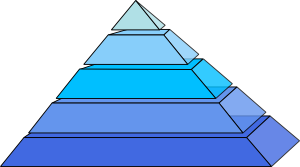
\includegraphics[width=1.1cm]{../Strukturfiler/FIGS/BluePyramid} & \begin{minipage}{\obsl}}{\end{minipage}\\ \end{tabular}\vspace{4mm}\newline}


% = Forudsætning = basis
\newenvironment{basis}{\begin{flushleft} \begin{itshape} }{\end{itshape} \end{flushleft}}


% = Opsummering =
\newenvironment{summary}{\clearpage\pagecolor{sumgul}\section{Opsummering}}{\newpage\pagecolor{white}}











% = Counter
\newcounter{opgavecount}[section]
\setcounter{opgavecount}{0}
\newcounter{spgcount}[opgavecount]
\setcounter{spgcount}{0}
\renewcommand{\thespgcount}{\alph{spgcount})}



% = EXERCISE = (DIVIDER)

\newcommand{\exercisebegin}[1][]{\bigskip\needspace{3\baselineskip}\refstepcounter{opgavecount}\titlegraphic{mingroen}\textcolor{mingroen}{\th{Opgave \theopgavecount \hspace*{1cm} #1}}\medskip\par}

% = QUIZEXERCISE = (DIVIDER)

\newcommand{\quizexercisebegin}[1][]{\bigskip\needspace{3\baselineskip}\refstepcounter{opgavecount}\titlegraphic{mingroen}\textcolor{mingroen}{\th{Quiz-Opgave \theopgavecount \hspace*{1cm} #1}}\medskip\par}

% = QUESTION =

\newenvironment{question}{\refstepcounter{spgcount}\begin{itemize}\item[\thespgcount]}{\end{itemize}\hspace*{\fill}}

% = VINK =

\newenvironment{vink}{\begin{tabular}{m{.9cm}<{\hspace*{2mm}}@{}|m{\obsl}@{}}\hspace*{-4pt}\raggedleft
\includegraphics[width=.9cm]{../Strukturfiler/FIGS/Think} & \begin{minipage}{\obsl}}{\end{minipage}\\ \end{tabular}\medskip\\}
	
% = FACIT =

\newenvironment{facit}{\begin{tabular}{m{.9cm}<{\hspace*{2mm}}@{}|m{\obsl}@{}}\hspace*{-4pt}\raggedleft
\includegraphics[width=.9cm]{../Strukturfiler/FIGS/Check} & \begin{minipage}{\obsl}}{\end{minipage}\\ \end{tabular}\medskip\\}








\newcommand{\afsnit}[1]{\bigskip\th{\titlegraphic{mingroen}\textcolor{mingroen}{#1}} \\ \rule[7pt]{.4\textwidth}{1pt} \vspace*{-2.5mm}\par}

% (DIVIDER):
\newcommand{\ugedagdatotitel}[4]{\pagebreak[4]\section{Semesteruge #1 -- #2 Dag \hspace*{1mm} (#3)} \vspace*{-4mm} \rule[5pt]{\textwidth}{1pt}\vspace*{-2.5mm} \begin{center}\large{\th{#4}}\end{center} \fancyhead[C]{\th{Semesteruge #1}}}

\newenvironment{skema}[1]{\definecolor{shadecolor}{rgb}{0.96,.98, 1.0} \setlength{\FrameSep}{6pt} \renewcommand{\FrameHeightAdjust}{10pt} \vspace*{-4pt}\begin{shaded} \begin{tabular}{#1}}{\end{tabular} \end{shaded} \vspace*{-7pt}}


% ========================

% MAKROER

%\newenvironment{matr}[1][]{\hspace*{-.8mm}\left[\hspace*{-1mm}\begin{array}{#1}}{\end{array}\hspace*{-1mm}\right]\hspace*{-.8mm}}
\newcommand{\bevisslut}{\begin{scriptsize} \begin{flushright} $ \blacksquare $ \end{flushright} \end{scriptsize}}

\newcommand{\tref}[2]{\hyperref[#1]{#2 \ref*{#1}}}
\newcommand{\thref}[2]{\hyperref[#1]{#2}}

\newcommand{\refA}[1]{\colorbox{yellow}{\ref{#1}}}
\newcommand{\hrefA}[2]{\colorbox{yellow}{\href{#1}{#2}}}
\newcommand{\trefA}[2]{\colorbox{yellow}{\hyperref[#1]{#2 \ref*{#1}}}}
\newcommand{\threfA}[2]{\colorbox{yellow}{\hyperref[#1]{#2}}}

\newenvironment{matr}[1]{\hspace*{-.8mm}\begin{bmatrix}\hspace*{-1mm}\begin{array}{#1}}{\end{array}\hspace*{-1mm}\end{bmatrix}\hspace*{-.8mm}}
\newcommand{\transp}{\hspace*{-.6mm}^{\top}}

\newcommand{\maengde}[2]{\left\lbrace \hspace*{-1mm} \begin{array}{c|c} #1 & #2 \end{array} \hspace*{-1mm} \right\rbrace}

\newenvironment{eqnalign}[1]{\setlength{\arraycolsep}{1.3pt}\begin{equation}\begin{array}{#1}}{\end{array}\end{equation}\par}
\newcommand{\eqnl}{\setlength{\arraycolsep}{1.3pt}}

\newcommand{\matind}[3]{{_\mathrm{#1}\mathbf{#2}_\mathrm{#3}}}
\newcommand{\vekind}[2]{{_\mathrm{#1}\mathbf{#2}}}
\newcommand{\jac}[2]{{\mathrm{Jacobi}_\mathbf{#1} (#2)}}
\newcommand{\diver}[2]{{\mathrm{div}\mathbf{#1} (#2)}}
\newcommand{\rot}[1]{{\mathbf{rot}\mathbf{(#1)}}}

\newcommand{\am}{\mathrm{am}}
\newcommand{\gm}{\mathrm{gm}}
\newcommand{\E}{\mathrm{E}}
\newcommand{\Span}{\mathrm{span}}
\newcommand{\mU}{\mathbf{U}}

\newcommand{\ms}{\medskip\\}
\newcommand{\bs}{\bigskip\\}

\newcommand{\mA}{\mathbf{A}}
\newcommand{\mB}{\mathbf{B}}
\newcommand{\mC}{\mathbf{C}}
\newcommand{\mD}{\mathbf{D}}
\newcommand{\mE}{\mathbf{E}}
\newcommand{\mF}{\mathbf{F}}
\newcommand{\mK}{\mathbf{K}}
\newcommand{\mI}{\mathbf{I}}
\newcommand{\mM}{\mathbf{M}}
\newcommand{\mN}{\mathbf{N}}
\newcommand{\mQ}{\mathbf{Q}}
\newcommand{\mT}{\mathbf{T}}
\newcommand{\mV}{\mathbf{V}}
\newcommand{\mW}{\mathbf{W}}
\newcommand{\mX}{\mathbf{X}}
\newcommand{\ma}{\mathbf{a}}
\newcommand{\mb}{\mathbf{b}}
\newcommand{\mc}{\mathbf{c}}
\newcommand{\md}{\mathbf{d}}
\newcommand{\me}{\mathbf{e}}
\newcommand{\mn}{\mathbf{n}}
\newcommand{\mr}{\mathbf{r}}
\newcommand{\mv}{\mathbf{v}}
\newcommand{\mw}{\mathbf{w}}
\newcommand{\mx}{\mathbf{x}}
\newcommand{\mxb}{\mathbf{x_{bet}}}
\newcommand{\my}{\mathbf{y}}
\newcommand{\mz}{\mathbf{z}}
\newcommand{\reel}{\mathbb{R}}
\newcommand{\mL}{\bm{\Lambda}} %Lambda-matrix
\newcommand{\mnul}{\bm{0}}
\newcommand{\trap}[1]{\mathrm{trap}(#1)}
\newcommand{\Det}{\operatorname{Det}}
\newcommand{\adj}{\operatorname{adj}}
\newcommand{\Ar}{\operatorname{Areal}}
\newcommand{\Vol}{\operatorname{Vol}}
\newcommand{\Rum}{\operatorname{Rum}}
\newcommand{\diag}{\operatorname{\bf{diag}}}
\newcommand{\bidiag}{\operatorname{\bf{bidiag}}}
\newcommand{\spanVec}[1]{\mathrm{span}\{#1\}}
\newcommand{\Div}{\operatorname{Div}}
\newcommand{\Rot}{\operatorname{\mathbf{Rot}}}

\newcommand{\Jac}{\operatorname{Jacobi}}
\newcommand{\Tan}{\operatorname{Tan}}
\newcommand{\Ort}{\operatorname{Ort}}
\newcommand{\Flux}{\operatorname{Flux}}
\newcommand{\Cmass}{\operatorname{Cm}}
\newcommand{\Imom}{\operatorname{Im}}
\newcommand{\Pmom}{\operatorname{Pm}}
\newcommand{\IS}{\operatorname{I}}
\newcommand{\IIS}{\operatorname{II}}
\newcommand{\IIIS}{\operatorname{III}}
\newcommand{\Le}{\operatorname{L}}
\newcommand{\app}{\operatorname{app}}
\newcommand{\M}{\operatorname{M}}
\newcommand{\re}{\mathrm{Re}}
\newcommand{\im}{\mathrm{Im}}

\newcommand{\compl}{\mathbb{C}} %de komplekse tal
\newcommand{\e}{\mathrm{e}} %eksponentialfunktionen. lodret 'e', og altså ikke kursiv ligesom andre bogstaver.





% Medialink: SCREEN: (QRcode) + thumbnail image + link på kodenummer (til qr.dtu.dk)
\newcommand{\onlinemedia}[3]{
	\begin{wrapfigure}{r}{3.2cm} 
		\vspace{-30pt} 
		\vspace{#1pt} 
		\begin{flushright} 
			\includegraphics[width=3cm]{qr/#2.png} 
			\tiny 
			\href{http://qr.dtu.dk/#2}{#2: #3}
			\normalsize  
		\end{flushright} 
		\vspace{-10pt} 
	\end{wrapfigure}
}
\newcommand{\onlinemediathumb}[3]{
	\begin{wrapfigure}{r}{3.2cm} 
		\vspace{-30pt} 
		\vspace{#1pt} 
		\begin{flushright} 
			\includegraphics[width=3cm]{qr/#2.png} 
			\includegraphics[width=3cm]{qr/#2_thumb.png} 
			\tiny 
			\href{http://qr.dtu.dk/#2}{#2: #3}
			\normalsize  
		\end{flushright} 
		\vspace{-10pt} 
	\end{wrapfigure}
}



% Index:
\usepackage{makeidx}
\makeindex
\newcommand\ind[2]{\index{#1}\textbf{\textit{\textcolor{black}{#2}}}}

% ###SERVER_EXCLUDE_BEGIN###
\externaldocument[NUID17-]{../../enoten/TN01-Talrum/Talrum}
\externaldocument[NUID1-]{../../enoten/TN02-Ligningssystemer/TNdriver}
\externaldocument[NUID2-]{../../enoten/TN03-Matricer_og_Matrixalgebra/Matricer_og_matrixalgebra}
\externaldocument[NUID3-]{../../enoten/TN04-Kvadratiske_matricer/TNdriver}
\externaldocument[NUID11-]{../../enoten/TN05-Determinanter/Determinanter}
\externaldocument[NUID12-]{../../enoten/TN06-GeometriskeVektorer/GeometriskeVektorer}
\externaldocument[NUID18-]{../../enoten/TN07-Vektorrum/VektorRum}
\externaldocument[NUID21-]{../../enoten/TN08-LinAfbildninger/LinAfbildninger}
\externaldocument[NUID23-]{../../enoten/TN09-Egenvaerdier_og_egenvektorer/TNdriver}
\externaldocument[NUID24-]{../../enoten/TN10-Diagonalisering_med_egenvektorer/TNdriver}
\externaldocument[NUID10-]{../../enoten/TN11-1.ordens_differentialligninger/TNdriver}
\externaldocument[NUID13-]{../../enoten/TN12-1.ordens_differentialligningssystemer/TNdriver}
\externaldocument[NUID14-]{../../enoten/TN13-2.ordens_differentialligninger/TNdriver}
\externaldocument[NUID27-]{../../enoten/TN14-Elemenataere_funktioner/Elementaere_Funktioner}
\externaldocument[NUID28-]{../../enoten/TN15-Funktioner2Variable/Funktioner_To_Variable}
\externaldocument[NUID29-]{../../enoten/TN16-Gradienter_og_Tangentplaner/Gradienter_og_Tangentplaner}
\externaldocument[NUID32-]{../../enoten/TN17-Taylor_formler/Taylor_Formler}
\externaldocument[NUID33-]{../../enoten/TN18-Taylor_2Var/Taylor_2Var}
\externaldocument[NUID34-]{../../enoten/TN19-SymMat/SymmetriskeMatricer}
\externaldocument[NUID35-]{../../enoten/TN20-KegleSnit/Keglesnit}
\externaldocument[NUID36-]{../../enoten/TN21-Riemann_Integral/Riemann_01}
\externaldocument[NUID37-]{../../enoten/TN22-Plan_Int/Plan_Int_01}
\externaldocument[NUID39-]{../../enoten/TN23-Flade_Int/Flade_Rum_Int_01}
\externaldocument[NUID40-]{../../enoten/TN24-Vektorfelter/Vektorfelter_01}
\externaldocument[NUID41-]{../../enoten/TN25-Flux/Flux_02}
\externaldocument[NUID42-]{../../enoten/TN26-Gauss/Gauss_01}
\externaldocument[NUID128-]{../../enoten/TN27-Stokes/Stokes_01}
\externaldocument[NUID43-]{../../enoten/TN29-KomplekseTal/KomplekseTal}

\externaldocument[NUID6-]{../../E-math-opgaver/Opgaver/opgU123}
\externaldocument[NUID19-]{../../E-math-opgaver/Opgaver/opgU45}
\externaldocument[NUID20-]{../../E-math-opgaver/Opgaver/opgU678}
\externaldocument[NUID25-]{../../E-math-opgaver/Opgaver/opgU910SD}
\externaldocument[NUID31-]{../../E-math-opgaver/OpgaverF11-U123/opgF123}
% \externaldocument[NUID9-]{../../E-math-opgaver/Opgaver/Dagsordner E10}
% ###SERVER_EXCLUDE_END###


% Begin document and set alternative chapter title:
\begin{document}
\renewcommand{\chaptername}{eNote}

\setcounter{chapter}{13} %SÆT DETTE TAL TIL 1 MINDRE END DET AKTUELLE TRANSFERNOTE-NUMMER!!

%%%%%%%%%%%%%%%%%%%%%%%%%%%%%%%%%%%%%%%%%%%%%
%%%%%%%%%%%%%%%%%%%%%%%%%%%%%%%%%%%%%%%%%%%%%
%%% HERFRA SKAL DU SKRIVE ELLER INDSÆTTE %%%%
%%% DEN FIL DU ØNSKER %%%%%%%%%%%%%%%%%%%%%%%
%%%%%%%%%%%%%%%%%%%%%%%%%%%%%%%%%%%%%%%%%%%%%
%%%%%%%%%%%%%%%%%%%%%%%%%%%%%%%%%%%%%%%%%%%%%


% REF: TransferNote \ref{TN4-tn4} \nameref{TN4-tn4}


\chapter{Elementære funktioner} \label{tn14}


\begin{basis}
I denne eNote vil vi dels repetere nogle af de basale egenskaber for et udvalg af de (fra gymnasiet) velkendte funktioner $f(x)$ af \'{e}n reel variabel $x$,  og dels introducere enkelte nye funktioner,
som typisk optræder i mangfoldige sammenhænge. De grundlæggende spørgsmål vedrørende enhver funktion drejer sig typisk om følgende: Hvordan og for hvilke $x$ er funktionen \emph{defineret}? Hvilke værdier af $f(x)$ får vi når vi bruger funktionen på elementerne $x$ i definitionsmængden? Er funktionen \emph{kontinuert}? Hvad er \emph{differentialkvotienten} $f'(x)$ af funktionen -- hvis den eksisterer? Som noget nyt vil vi indføre en meget stor \emph{klasse} af funktioner, \ind{epsilon-funktioner}{epsilon-funktionerne}, som betegnes med fællesbetegnelsen $\varepsilon(x)$ og som vi gennemgående vil benytte til at beskrive kontinuitet og differentiabilitet -- også af funktioner af flere variable, som vil blive indført og analyseret i de efterfølgende eNoter.
\end{basis}


%%%%%%%%%%%%%%%%%%%%%%%%%%%%%%%%%%%%%%%%%%%%%%%%%%%%%%%%%%%%%
%%%%%%%%%%%%%%%%%%%%%%%%%%%%%%%%%%%%%%%%%%%%%%%%%%%%%%%%%%%%%
%%%%%%%%%%%%%%%%%%%%%%%%%%%%%%%%%%%%%%%%%%%%%%%%%%%%%%%%%%%%%



\section{Definitionsmængde og værdimængde} \label{tn14.secDefVal}
Ved beskrivelsen af en reel funktion $f(x)$ anføres dels de reelle tal $x$, hvor funktionen er defineret, og dels de
værdier, som kan fås ved at benytte funktionen på defintionsmængden. \ind{definitionsmængde}{Definitionsmængden} kalder vi $\mathcal{D}m(f)$ og \ind{værdimængde}{værdimængden} kalder vi $\mathcal{V}m(f)$.

\begin{example}[Nogle definitionsmængder og værdimængder] \label{tn14.exampElemDV}
Her er  definitonsmængder og tilhørende værdimængder for nogle velkendte funktioner.
\begin{equation}
\begin{array}{lllll}
  f_{1}(x) = \exp(x) & , & \mathcal{D}m(f_{1}) = \mathbb{R} = \, ]- \infty, \infty[  & , & \mathcal{V}m(f_{1}) = \,]0, \infty[ \\
  f_{2}(x) = \ln(x) & , & \mathcal{D}m(f_{2}) =  ]0, \infty[  & , & \mathcal{V}m(f_{2}) = \mathbb{R} = \, ]- \infty, \infty[  \\
  f_{3}(x) = \sqrt{x} & , & \mathcal{D}m(f_{3}) = \, [0, \infty[  & , & \mathcal{V}m(f_{3}) = \,[0, \infty[ \\
  f_{4}(x) = x^{2} & , & \mathcal{D}m(f_{4}) = \mathbb{R} = \, ]- \infty, \infty[  & , & \mathcal{V}m(f_{4}) = \,[0, \infty[ \\
  f_{5}(x) = x^{7}+ 8x^{3} + x -1 & , & \mathcal{D}m(f_{5}) = \mathbb{R} = \, ]- \infty, \infty[  & , & \mathcal{V}m(f_{5}) = \mathbb{R} = \, ]- \infty, \infty[ \\
  f_{6}(x) = \exp(\ln(x))& , & \mathcal{D}m(f_{6}) =  \, ]0, \infty[  & , & \mathcal{V}m(f_{6}) = \, ]0, \infty[  \\
  f_{7}(x) = \sin(1/x) & , & \mathcal{D}m(f_{7}) = \, ]- \infty, 0[ \cup ]0, \infty[  & , & \mathcal{V}m(f_{7}) = [-1, 1]\\
  f_{8}(x) = |x|/x & , & \mathcal{D}m(f_{8}) = \, ]- \infty, 0[ \cup ]0, \infty[  & , & \mathcal{V}m(f_{8}) = \{-1\} \cup \{1\} \\
\end{array}
\end{equation}
\end{example}


\begin{figure}[h]
\centerline{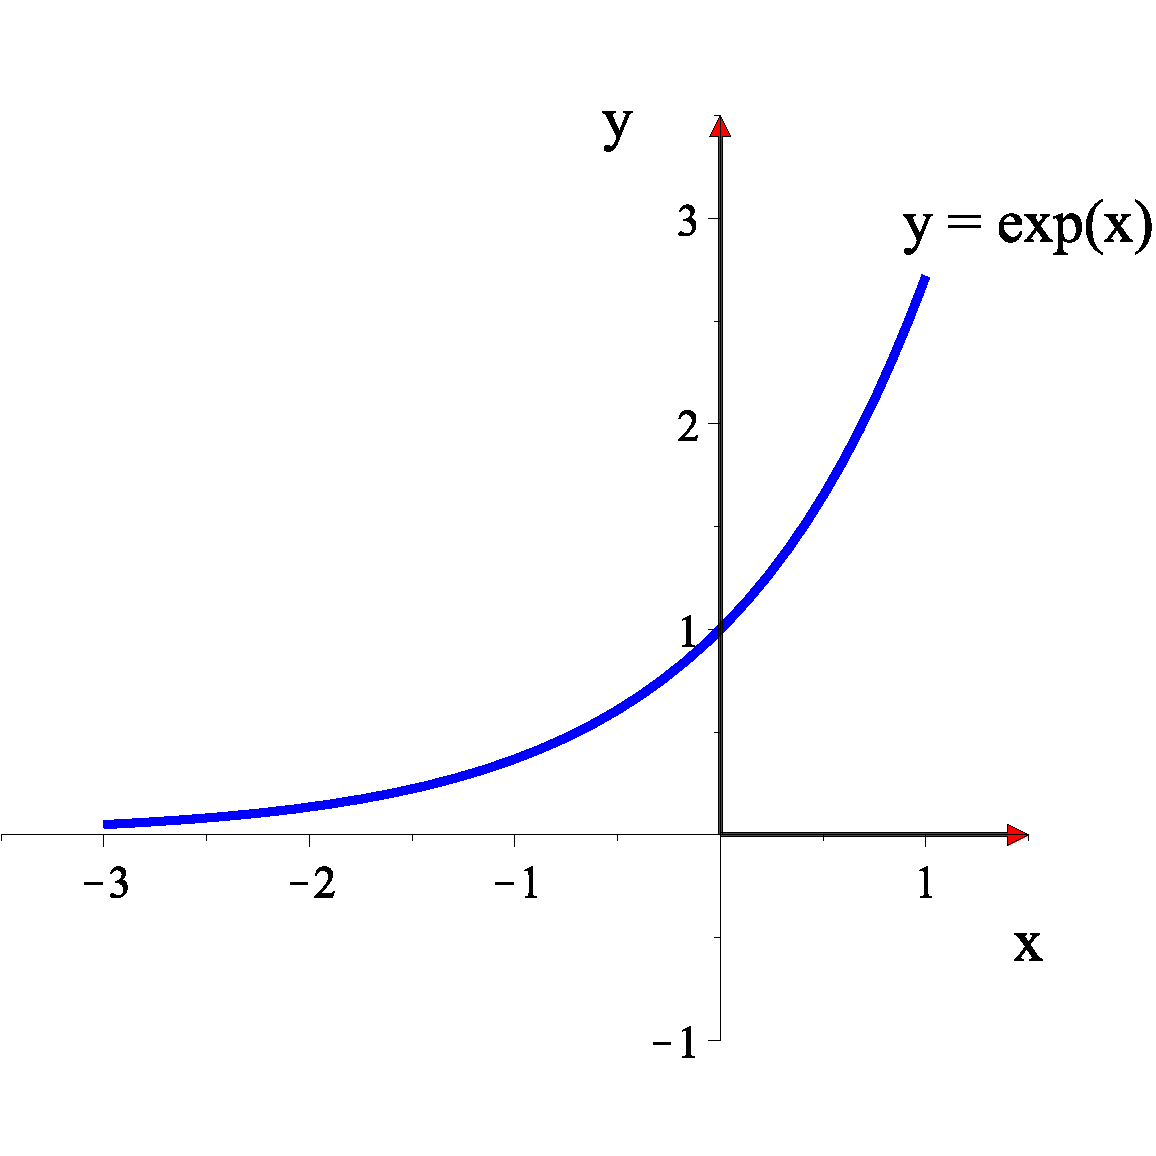
\includegraphics[width=75mm]{FIGS/plotexp02.pdf} 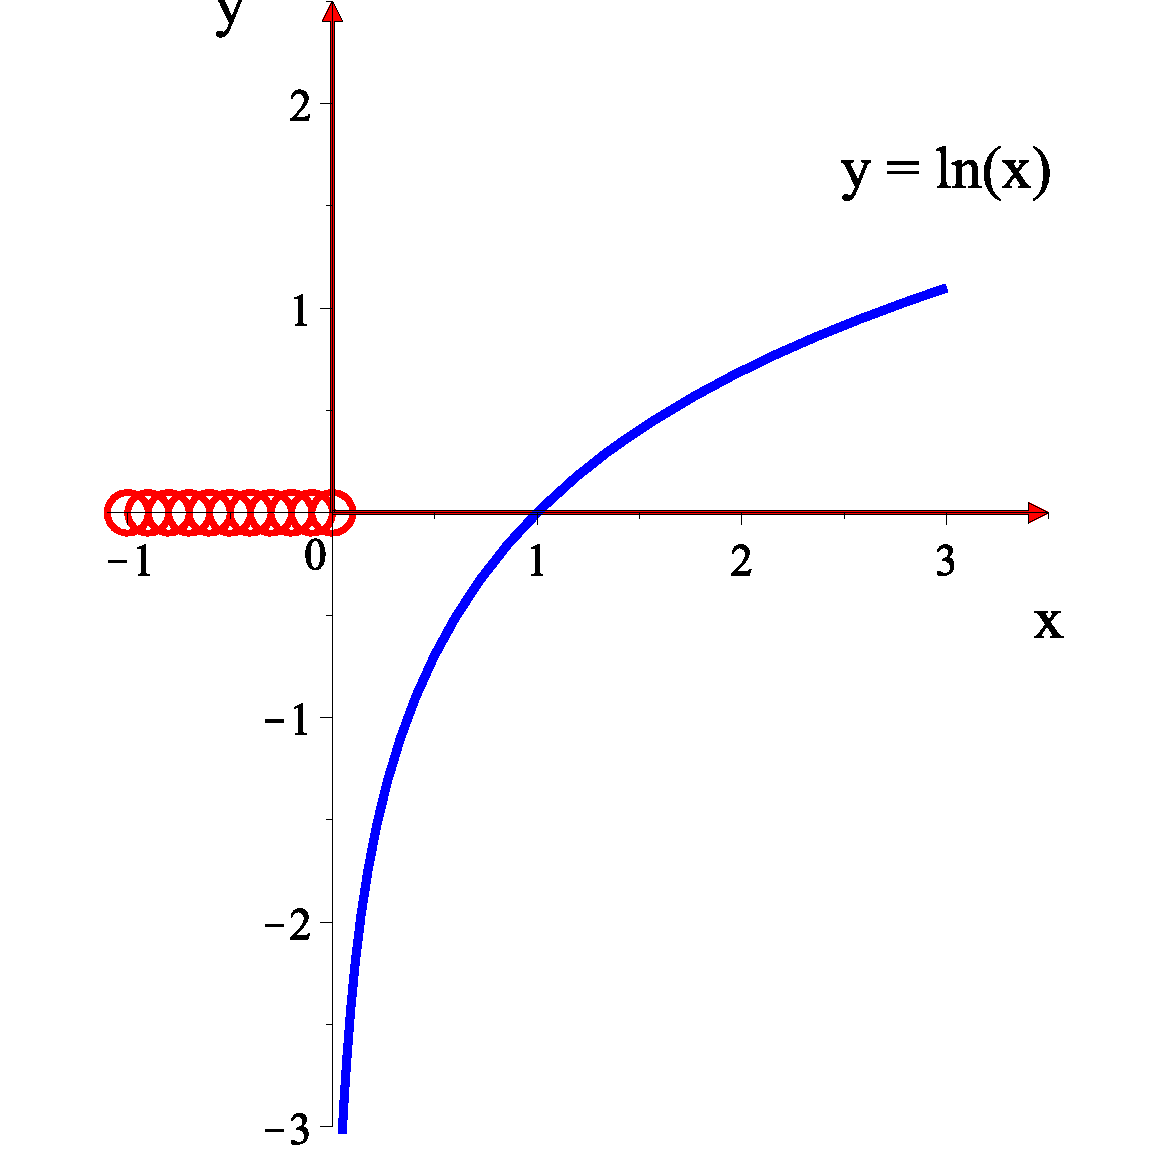
\includegraphics[width=75mm]{FIGS/plotln.pdf}}
\begin{center}
\caption{Den velkendte eksponentialfunktion $e^{x} = \exp(x)$ og den naturlige logaritmefunktion $\ln(x)$. De røde cirkler på den negative $x$-akse og i $0$ indikerer, at logaritmefunktionen ikke er defineret i $]-\infty, 0]$. } \label{tn14.figExpLn}
\end{center}
\end{figure}



\begin{think}
Funktionen $f_{8}(x)$ i eksempel \ref{tn14.exampElemDV} er defineret ud fra $|x|$, som betegner den numeriske værdi af $x$, dvs.
\begin{equation}
|x| = \left\{
        \begin{array}{ll}
          x > 0 \, \, , & \hbox{for} \quad x > 0 \\
          0 \, \,, & \hbox{for} \quad x = 0 \\
          -x >0 \, \,, & \hbox{for} \quad x < 0  \quad.
        \end{array}
      \right.
\end{equation}
Heraf følger definitionsmængde og værdimængde for $f_{8}(x)$ direkte.
\end{think}

\begin{example}[Tangens]
Funktionen
\begin{equation}
f(x) = \tan(x) = \frac{\sin(x)}{\cos(x)}
\end{equation}
har definitionsmængden $\mathcal{D}m(f) = \mathbb{R} \setminus A$, hvor $A$ betegner de reelle tal $x$, hvor nævneren $\cos(x)$ er $0$, dvs.
\begin{equation}
\mathcal{D}m(f) =  \mathbb{R} \setminus \{ x\,| \, \cos(x) = 0 \} = \mathbb{R} \setminus \{(\pi/2) + p \cdot \pi \, , \, \textrm{hvor $p$ er et helt tal} \}\quad.
\end{equation}
Værdimængden $\mathcal{V}m(f)$ er alle de reelle tal, se figur \ref{tn14.figplottancot}.
\end{example}

\begin{figure}[h]
\centerline{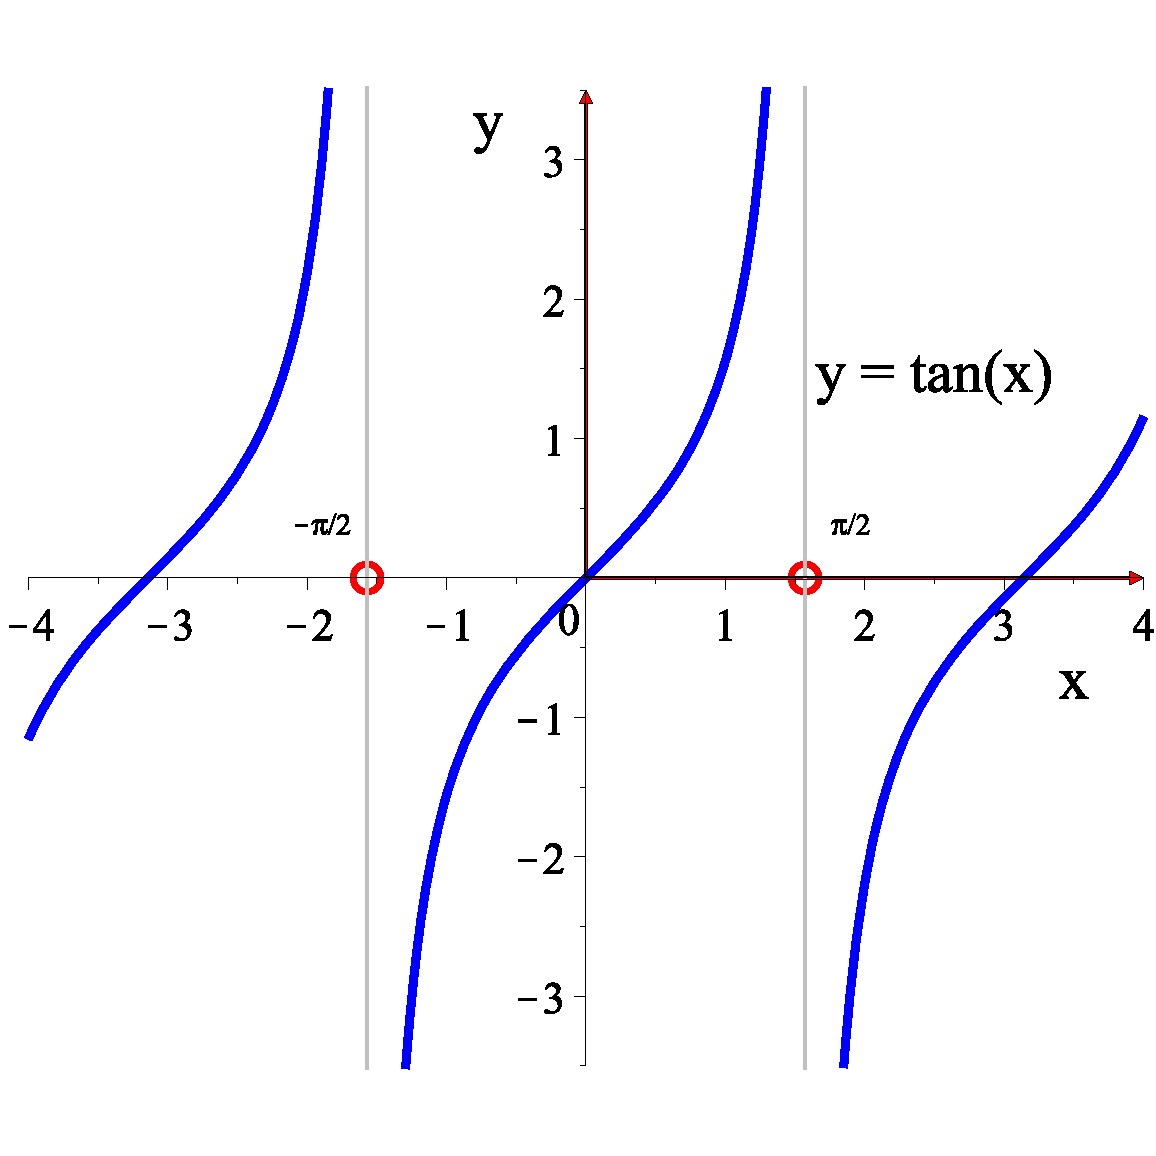
\includegraphics[height=70mm]{FIGS/plottan.pdf} \quad \quad \quad 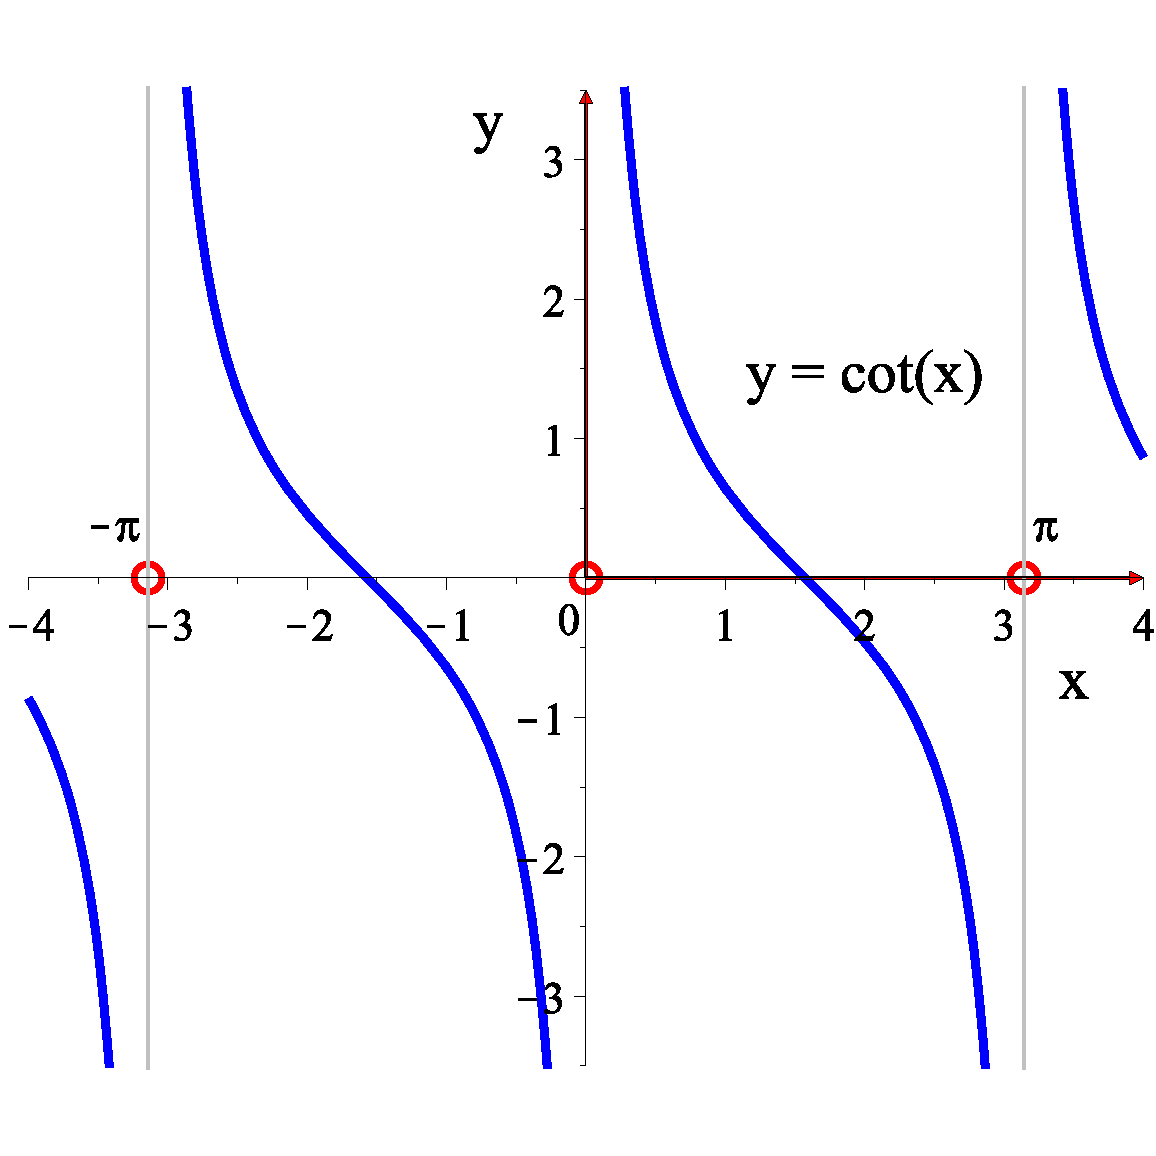
\includegraphics[height=70mm]{FIGS/plotcot.pdf}}
\begin{center}
\caption{Graferne for funktionerne $\tan(x)$ og $\cot(x)$.} \label{tn14.figplottancot}
\end{center}
\end{figure}




\begin{exercise}
Lad $g(x)$ betegne den reciprokke funktion til funktionen $\tan(x)$:
\begin{equation}
g(x) = \cot(x) = \frac{\cos(x)}{\sin(x)}
\end{equation}
Bestem definitionsmængden for $g(x)$ og skriv den på samme måde som for $\tan(x)$ ovenfor, se figur \ref{tn14.figplottancot}.
\end{exercise}

%%%%%%%%%%%%%%%%%%%%%%%%%%%%%%%%%%%%%%%%%%%%%%%%%%%
%%%%%%%%%%%%%%%%%%%%%%%%%%%%%%%%%%%%%%%%%%%%%%%%%%%


\subsection{Udvidelser af definitionsmængden til hele $\mathbb{R}$}

En funktion $f(x)$, som ikke er defineret i alle reelle tal, kan kan let \emph{udvides} til en funktion $\widehat{f}(x)$ som  har $\mathcal{D}m(\widehat{f}) = \mathbb{R}$. Det kan for eksempel gøres ved hjælp af en \ind{tuborgparentes}{tuborgparentes} på følgende måde:

\begin{definition}
Givet en funktion $f(x)$ med $\mathcal{D}m(f) \neq \mathbb{R}$, så definerer vi \ind{nul-udvidelse af en funktion}{$0$-udvidelsen} af $f(x)$ ved:
\begin{equation}
\widehat{f}(x) = \left\{
                      \begin{array}{ll}
                        f(x)\, , & \hbox{for} \quad x \in \mathcal{D}m(f)\\
                        0 \, , & \hbox{for} \quad  x \in \mathbb{R} \setminus \mathcal{D}m(f) \quad .
                      \end{array}
                    \right.
\end{equation}
\end{definition}

\begin{think}
Det er klart, at afhængig af anvendelsen kan man plombere og udvide definitionsmængden for $f(x)$ på mange andre måder end ved at vælge konstanten $0$ som værdi for den udvidede funktion i de punkter hvor den oprindelige funktion ikke er defineret.
\end{think}

\begin{aha}
\emph{Værdimængden} $\mathcal{V}m(\widehat{f})$ for den $0$-udvidede funktion er naturligvis den oprindelige værdimængde for $f(x)$ forenet med værdien $0$, dvs. $\mathcal{V}m(\widehat{f}) = \mathcal{V}m(f) \cup \{0\}$ .
\end{aha}


Vi vil herefter typisk -- medmindre andet nævnes helt tydeligt -- antage, at de funktioner vi betragter er definerede i hele $\mathbb{R}$ (eventuelt ved hjælp af en udvidelseskonstruktion) som ovenfor.


%%%%%%%%%%%%%%%%%%%%%%%%%%%%%%%%%%%%%%%%%%%%%%%%%%%%%%%%%%%%%
%%%%%%%%%%%%%%%%%%%%%%%%%%%%%%%%%%%%%%%%%%%%%%%%%%%%%%%%%%%%%
%%%%%%%%%%%%%%%%%%%%%%%%%%%%%%%%%%%%%%%%%%%%%%%%%%%%%%%%%%%%%


\section{Epsilon-funktioner} \label{tn14.secOmvendtFunk}

Vi indfører en særlig klasse af funktioner, som vi vil benytte til at definere
det vigtige begreb kontinuitet for funktioner.

\begin{definition}[Epsilon-funktioner] \label{tn14.defEpsilonFunk}
 Enhver funktion $\varepsilon(x)$ som er defineret i et åbent interval der indeholder $0$,
 og som antager værdien $\varepsilon(0) = 0$ i $x=0$ og
 derudover går imod $0$ når $x$ går imod $0$ kaldes en \ind{epsilon-funktion}{epsilon-funktion} af $x$. Epsilon-funktioner er altså karakteriserede ved egenskaberne:
 \begin{equation}
 \varepsilon(0) = 0 \quad \textrm{og} \quad  \varepsilon(x) \to 0 \quad \textrm{for} \quad x \to 0 \quad .
 \end{equation}
Den sidste betingelse er ækvivalent med, at den numeriske værdi af $\varepsilon(x)$ kan gøres så lille som ønsket ved blot at vælge den numeriske værdi af $x$ tilstrækkelig lille. Helt præcis betyder betingelsen:
For ethvert helt tal $k >0$ findes der et helt tal $K > 0$ sådan at $|\varepsilon(x)| < 1/k$ for alle $x$ med  $|x| < 1/K$.\\
\end{definition}

Mængden af epsilon-funktioner er meget stor:

\begin{example}[Epsilon-funktioner]
Her er nogle simple eksempler på epsilon-funktioner:
\begin{equation}
\begin{aligned}
\varepsilon_{1}(x) &=  x\\
\varepsilon_{2}(x) &=  |x| \\
\varepsilon_{3}(x) &= \ln(1+x) \\
\varepsilon_{4}(x) &= \sin(x) \quad .\\
\end{aligned}
\end{equation}
\end{example}

\begin{aha}
Egenskaben 'at være en epsilon-funktion' er ret stabil:
Produktet af en epsilon-funktion med en vilkårlig anden funktion, der blot er begrænset, er også en epsilon-funktion.
Summen og produktet af to epsilon-funktioner er  igen epsilon-funktioner. Den numeriske værdi
af en epsilon-funktion er en epsilon-funktion.
\end{aha}

Funktioner der er $0$ andre steder end i $x=0$ kan også give anledning til epsilon-funktioner:

\begin{think}
Hvis en funktion $g(x)$ har egenskaberne $g(x_{0}) = 0$ og  $g(x) \to 0$ for $x \to x_{0}$, så er $g(x)$ en epsilon-funktion af $x-x_{0}$, dvs. vi kan skrive $g(x) = \varepsilon_{g}(x-x_{0})$.
\end{think}

\begin{exercise} \label{tn14.exercNumDiv}
Vis, at $0$-udvidelsen $\widehat{f}_{8}(x)$ af funktionen $f_{8}(x) = |x|/x$ \emph{ikke} er en epsilon-funktion. Vink: Hvis vi vælger $k = 10$ så findes der helt klart \emph{ikke} nogen værdi af $K$ sådan at
\begin{equation}
|f_{8}(x)| = |\,|x|/x \,| = 1 < \frac{1}{10}\quad , \quad \textrm{for alle $x$ med} \quad  |x| < \frac{1}{K}\quad .
\end{equation}
Tegn grafen for $\widehat{f}_{8}(x)$. Den kan ikke tegnes uden at 'løfte blyanten fra papiret'!
\end{exercise}


\begin{exercise} \label{tn14.exercSinusWild}
Vis, at $0$-udvidelsen af funktionen $f(x) = \sin(1/x)$ \emph{ikke} er en epsilon-funktion.
\end{exercise}


%%%%%%%%%%%%%%%%%%%%%%%%%%%%%%%%%%%%%%%%%%%%%%%%%%%%%%%%%%%%%
%%%%%%%%%%%%%%%%%%%%%%%%%%%%%%%%%%%%%%%%%%%%%%%%%%%%%%%%%%%%%
%%%%%%%%%%%%%%%%%%%%%%%%%%%%%%%%%%%%%%%%%%%%%%%%%%%%%%%%%%%%%


\section{Kontinuerte funktioner} \label{tn14.secDifferentiation}

Vi kan nu formulere \ind{kontinuitetsbegrebet}{kontinuitetsbegrebet} ved hjælp af epsilon-funktioner:

\begin{definition}[Kontinuitet] \label{tn14.defKont}
En funktion $f(x)$ er kontinuert i $x_{0}$ hvis der eksisterer en
epsilon-funktion $\varepsilon_{f}(x - x_{0})$ således at følgende gælder i et åbent interval der indeholder $x_{0}$:
\begin{equation}
f(x) = f(x_{0}) + \varepsilon_{f}(x - x_{0}) \quad .
\end{equation}
Hvis $f(x)$ er kontinuert i alle $x_{0}$ i et givet åbent interval i $\mathcal{D}m(f)$, så siger vi at $f(x)$ er kontinuert i intervallet.
\end{definition}

\begin{aha}
Læg mærke til, at selv om det klart, hvad epsilon-funktionen helt præcist er i definitionen \ref{tn14.defKont}, nemlig $f(x) - f(x_{0})$, så er den eneste egenskab vi er interesserede i følgende:
$\varepsilon_{f}(x - x_{0}) \to 0$ for $ x \to {0}$, sådan at $f(x) \to f(x_{0})$ for $x \to x_{0}$,
altså præcis som vi kender kontinuitets-begrebet fra gymnasiet!
\end{aha}

\begin{exercise} \label{tn14.exercNonKontEps}
Alle epsilon-funktioner er herefter per definition kontinuerte i $x_{0} = 0$ (med værdien $0$ i $x_{0}=0$). Konstru\'{e}r en epsilon-funktion, som \emph{ikke} er kontinuert i nogen som helst af punkterne $x_{0} = 1/n$ hvor $n = 1, 2, 3, 4, \cdots$.
\end{exercise}

\begin{aha}
Selvom epsilon-funktions-begrebet er helt fundamentalt for definitionen af kontinuitet (og, som vi skal se nedenfor, for definitionen af differentiabilitet), så behøver epsilonfunktionerne altså ikke selv at være kontinuerte andre steder end netop i $x_{0}=0$.
\end{aha}

\begin{exercise} \label{tn14.exercNumDiv}
Vis, at $0$-udvidelsen $\widehat{f}(x)$ af funktionen $f(x) = |x-7|/(x-7)$ \emph{ikke} er kontinuert i $\mathbb{R}$.
\end{exercise}

%%%%%%%%%%%%%%%%%%%%%%%%%%%%%%%%%%%%%%%%%%%%%%%%%%%%%%%%%%%%%
%%%%%%%%%%%%%%%%%%%%%%%%%%%%%%%%%%%%%%%%%%%%%%%%%%%%%%%%%%%%%
%%%%%%%%%%%%%%%%%%%%%%%%%%%%%%%%%%%%%%%%%%%%%%%%%%%%%%%%%%%%%


\section{Differentiable funktioner} \label{tn14.secDifferentiation}
\begin{definition}[Differentiabilitet]
En funktion $f(x)$ er differentiabel i $x_{0} \in \mathcal{D}m(f)$ hvis der findes en konstant $a$ og en epsilon-funktion $\varepsilon_{f}(x-x_{0})$ sådan at
\begin{equation} \label{tn14.eqDifferentiabilitet}
f(x) = f(x_{0}) + a\cdot(x-x_{0}) + (x-x_{0})\cdot \varepsilon_{f}(x-x_{0}) \quad.
\end{equation}
Det er det tal $a$, vi kalder $f'(x_{0})$ og det er veldefineret i den forstand, at hvis $f(x)$ i det hele taget \emph{kan} fremstilles på ovenstående form
(altså hvis $f(x)$ er differentiabel i $x_{0}$), så er der \'{e}n og kun \'{e}n værdi for $a$, som gør formlen rigtig. Med denne definition af \ind{differentialkvotient}{differentialkvotienten} $f'(x_{0})$ af $f(x)$ i $x_{0}$ har vi altså:
\begin{equation} \label{tn14.eqDifferentiabilitetB}
f(x) = f(x_{0}) + f'(x_{0})\cdot(x-x_{0}) + (x-x_{0})\cdot \varepsilon_{f}(x-x_{0}) \quad.
\end{equation}
Hvis $f(x)$ er differentiabel i alle $x_{0}$ i et givet åbent interval i $\mathcal{D}m(f)$, så siger vi naturligvis, at $f(x)$ er differentiabel i intervallet.
Vi skriver ofte differentialkvotienten af $f(x)$ i $x$ på følgende alternative måde:
\begin{equation}
f'(x) = \frac{d}{dx}f(x) \quad .
\end{equation}
\end{definition}

\begin{explain}[Differentialkvotienten er entydig]
Vi vil vise, at der kun findes \'{e}n værdi af $a$, som kan opfylde ligningen (\ref{tn14.eqDifferentiabilitet}). Antag nemlig, at der var to forskellige værdier, $a_{1}$ og $a_{2}$ som opfylder ligning (\ref{tn14.eqDifferentiabilitet}) med muligvis to forskellige epsilon-funktioner:
\begin{equation} \label{tn14.eqDichotomy}
\begin{aligned}
f(x) &= f(x_{0}) + a_{1}\cdot(x-x_{0}) + (x-x_{0})\cdot \varepsilon_{1}(x-x_{0}) \\
f(x) &= f(x_{0}) + a_{2}\cdot(x-x_{0}) + (x-x_{0})\cdot \varepsilon_{2}(x-x_{0}) \quad.
\end{aligned}
\end{equation}
Ved at trække nederste ligning i (\ref{tn14.eqDichotomy}) fra den øverste ligning får vi så:
\begin{equation}
0 = 0 + (a_{1} - a_{2})\cdot(x-x_{0}) + (x-x_{0})\cdot \left(\varepsilon_{1}(x-x_{0}) -  \varepsilon_{2}(x-x_{0})\right) \quad ,
\end{equation}
således at
\begin{equation}
a_{1} - a_{2} = \varepsilon_{1}(x-x_{0}) -  \varepsilon_{2}(x-x_{0})
\end{equation}
for alle $x \neq x_{0}$ -- og det kan klart ikke være rigtigt; højresiden går jo imod $0$ når $x$ går imod $x_{0}$! Antagelsen ovenfor, altså at $a_{1} \neq a_{2}$,  er derfor forkert. De to konstanter $a_{1}$ og $a_{2}$ må være ens, og det var det vi skulle indse.
\end{explain}

\begin{aha}
Ovenstående definition er helt ækvivalent med den vi kender fra gymnasiet. Hvis vi nemlig først trækker $f(x_{0})$ fra begge sider af lighedstegnet i ligning (\ref{tn14.eqDifferentiabilitetB}) og dernæst dividerer med $(x - x_{0})$   får vi
\begin{equation}
\frac{f(x) - f(x_{0})}{x - x_{0}} = f'(x_{0}) + \varepsilon_{f}(x-x_{0}) \to f'(x_{0}) \quad \textrm{for} \quad x \to x_{0} \quad ,
\end{equation}
altså den velkendte grænseværdi for \emph{kvotienten} mellem funktionstilvæksten $f(x) - f(x_{0})$ og $x$-tilvæksten $x - x_{0}$. Grunden til, at vi ikke bruger denne
kendte de\-fi\-ni\-tion af $f'(x_{0})$ er den simple, at for funktioner af flere variable giver kvotient-brøken ikke mening -- men mere om det i en senere eNote.
\end{aha}

\begin{theorem}[Differentiabel medfører kontinuert]
Hvis en funktion $f(x)$ er differentiabel i $x_{0}$, så er $f(x)$ også kontinuert i $x_{0}$.
\end{theorem}
\begin{bevis}
Vi har at
\begin{equation}
\begin{aligned}
f(x)&= f(x_{0}) + f'(x_{0})\cdot(x-x_{0}) + (x-x_{0})\varepsilon_{f}(x-x_{0})\\
 &= f(x_{0}) + \left[ f'(x_{0})\cdot(x-x_{0}) + (x-x_{0})\varepsilon_{f}(x-x_{0})\right],
\end{aligned}
\end{equation}
og da den kantede parentes på højre side er en epsilon-funktion af $(x - x_{0})$ så er $f(x)$ kontinuert i $x_{0}$.
\end{bevis}

Men det omvendte gælder ikke -- her er et eksempel, der viser det:
\begin{example}[Kontinuert men ikke differentiabel]
Funktionen $f(x) = |x|$ er kontinuert men ikke differentabel i $x_{0} = 0$. Funktionen er selv en epsilon-funktion og $f(x)$ er derfor
kontinuert i $0$. Men antag nu, at der findes en konstant $a$ og en epsilon-funktion $\varepsilon_{f}(x-x_{0})$ sådan at
\begin{equation}
f(x) = f(x_{0}) + a\cdot(x-x_{0}) + (x-x_{0})\varepsilon_{f}(x-x_{0}) \quad .
\end{equation}
Det vil sige, at så skulle der gælde:
\begin{equation}
|x|  = 0 + a\cdot x + x \cdot \varepsilon_{f}(x)
\end{equation}
og dermed for alle $x \neq 0$:
\begin{equation}
\frac{|x|}{x}  = a + \varepsilon_{f}(x) \quad .
\end{equation}
Det kan ikke lade sig gøre, for så skulle $a$ være både $-1$ og $1$ og det er umuligt! Derfor er ovenstående antagelse om, at der skulle findes
en sådan konstant $a$ altså forkert; $f(x)$ er derfor ikke differentiabel.
\end{example}


\begin{definition}
Det approksimerende første-grads-polynomium for $f(x)$ med udviklingspunkt $x_{0}$ defineres ved:
\begin{equation}
P_{1, x_{0}}(x) = f(x_{0}) + f'(x_{0})\cdot(x - x_{0}) \quad .
\end{equation}

\end{definition}

\begin{aha}
Bemærk, at $P_{1, x_{0}}(x)$ virkelig \emph{er} et første-gradspolynomium i $x$.
Grafen for funktionen $P_{1, x_{0}}(x)$ er \ind{tangenten til grafen}{tangenten til grafen} for $f(x)$ igennem punktet $(x_{0}, f(x_{0}))$, se figur \ref{tn14.figP1}. Ligningen for tangenten er $y = P_{1, x_{0}}(x)$, altså $y = f(x_{0}) + f'(x_{0})\cdot(x-x_{0})$. Hældningskoefficienten for tangenten er klart
$\alpha = f'(x_{0})$ og tangenten skærer $y$-aksen i punktet $(0, f(x_{0})-x_{0}\cdot f'(x_{0}))$. Vi skal senere finde ud af, hvordan vi kan approksimere med polynomier af højere grad $n$, altså polynomier der så betegnes $P_{n, x_{0}}(x)$.
\end{aha}

\begin{figure}[h]
\centerline{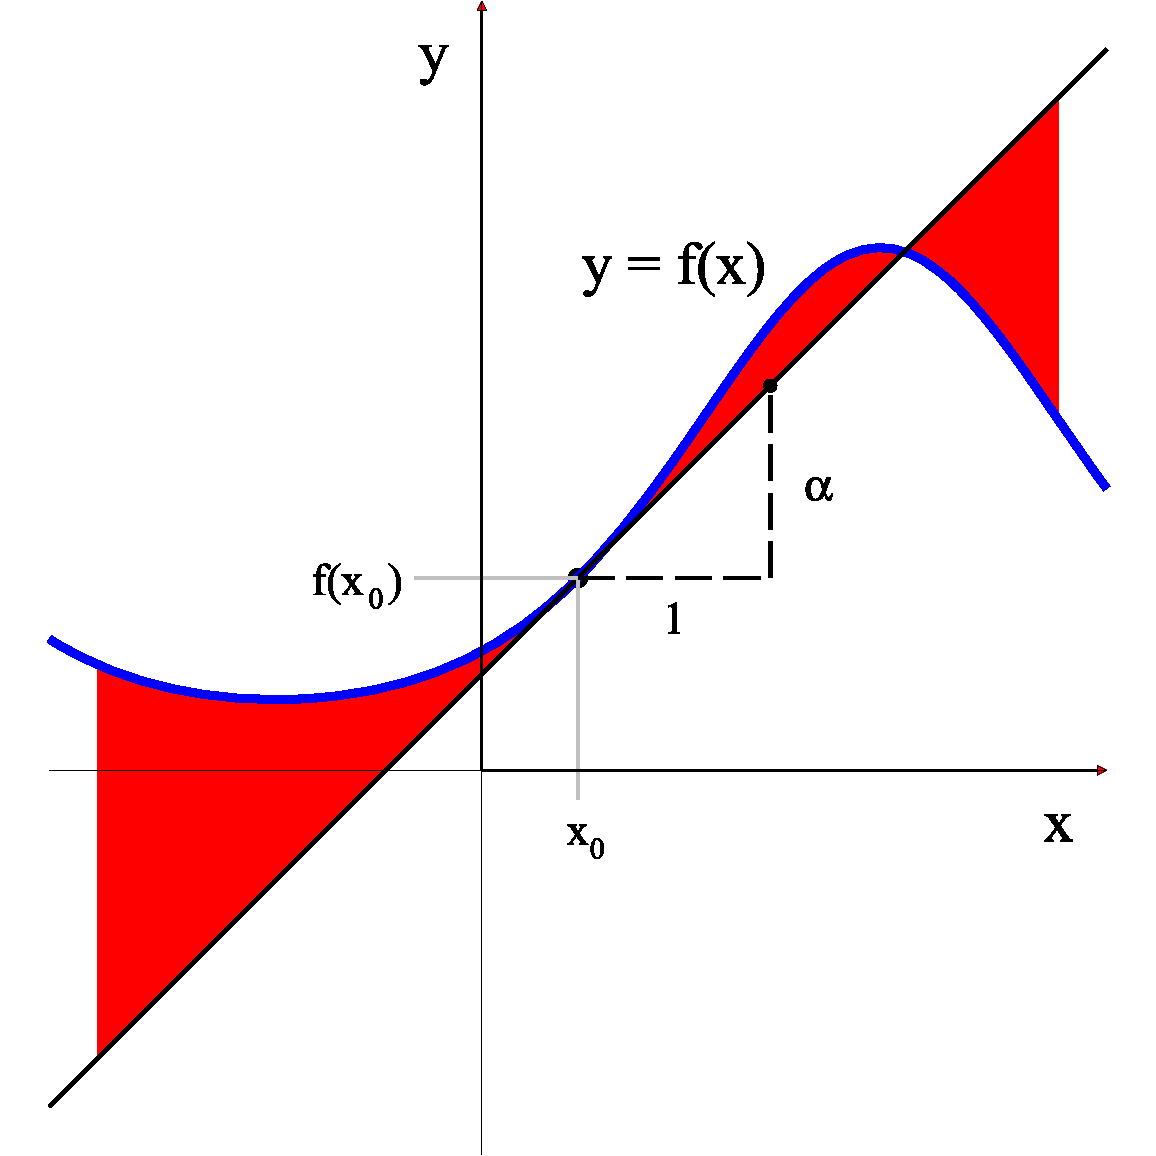
\includegraphics[height=70mm]{FIGS/plotEpsilon1.pdf}\qquad 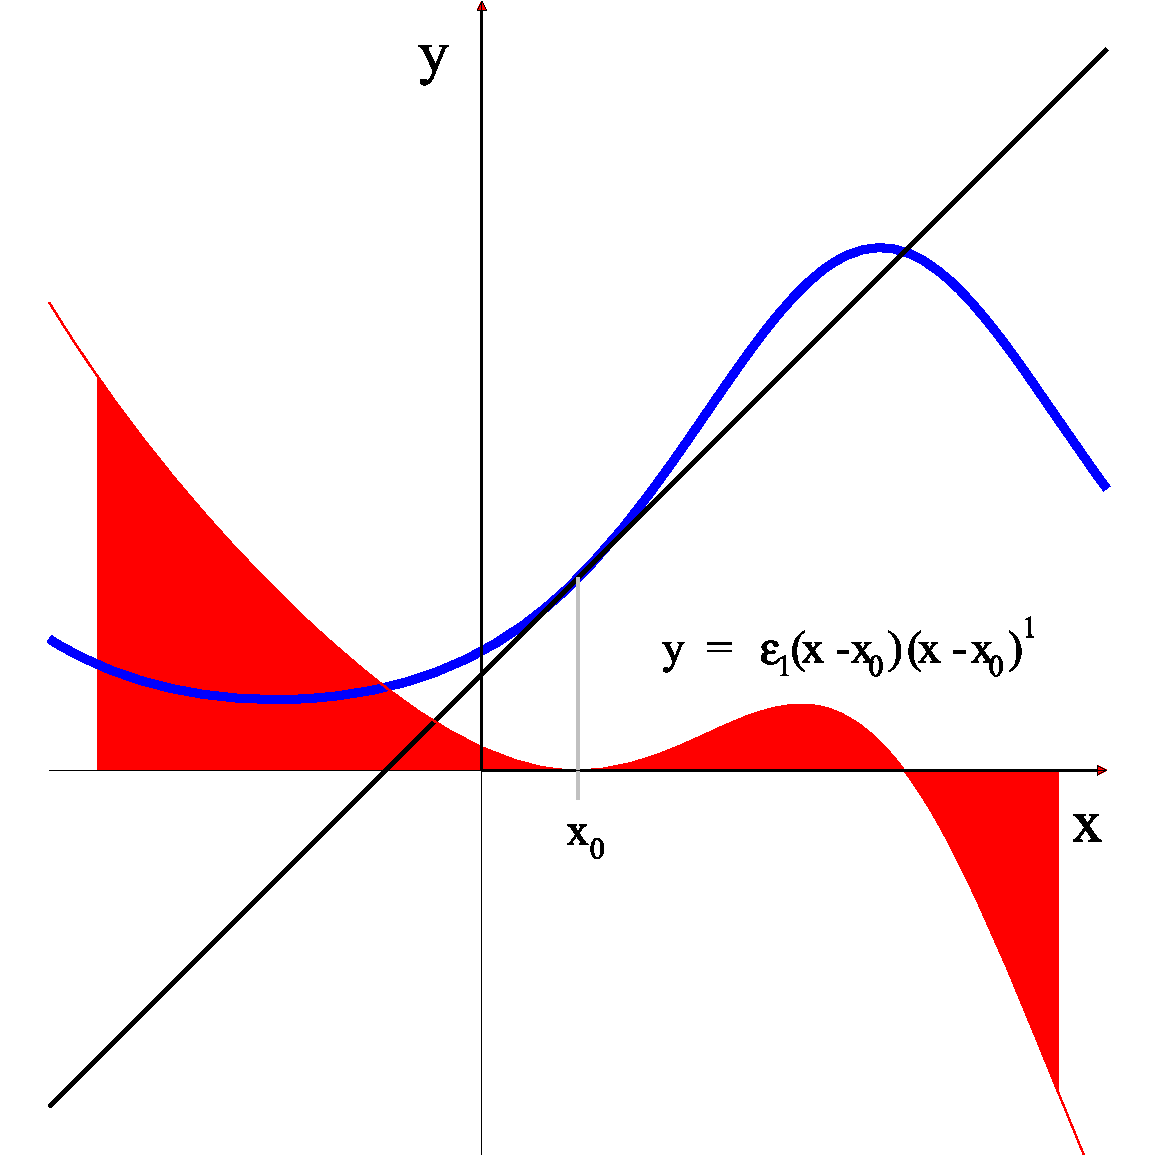
\includegraphics[height=70mm]{FIGS/plotEpsilon1Pur.pdf}}
\begin{center}
\caption{Konstruktion af tangenten $y = P_{1, x_{0}}(x) = f(x_{0}) +  \alpha\cdot(x-x_{0})$ med hældningskoefficienten $\alpha = f'(x_{0})$ for funktionen $f(x)$. Til højre ses forskellen mellem funktionsværdien $f(x)$ og 'tangentværdien' $P_{1, x_{0}}(x)$.} \label{tn14.figP1}
\end{center}
\end{figure}


%%%%%%%%%%%%%%%%%%%%%%%%%%%%%%%%%%%%%%%%%%%%%%%%%%%%%%%%%%%%%
%%%%%%%%%%%%%%%%%%%%%%%%%%%%%%%%%%%%%%%%%%%%%%%%%%%%%%%%%%%%%


\subsection{Differentiation af et produkt}
\begin{theorem}[Differentiation af $f(x)\cdot g(x)$]
Et produkt $h(x) = f(x) \cdot g(x)$ af  to differentiable funktioner $f(x)$ og $g(x)$ er differentiabel og differentieres på følgende velkendte måde:
\begin{equation}
\frac{d}{dx}\left(f(x)\cdot g(x)\right) = f'(x)\cdot g(x) + f(x)\cdot g'(x) \quad .
\end{equation}
\end{theorem}

Selv om denne formel formentlig er ganske velkendt fra gymnasiet, vil vi kort skitsere et bevis for den igen -- for at illustrere brugen af epsilon-funktioner.
\begin{bevis}
Vi har altså, da $f(x)$ og $g(x)$ er differentiable i $x_{0}$:
\begin{equation}
\begin{aligned}
f(x) &= f(x_{0}) + f'(x_{0})\cdot (x - x_{0}) + (x - x_{0})\varepsilon_{f}(x-x_{0}) \\
g(x) &= g(x_{0}) + g'(x_{0})\cdot (x - x_{0}) + (x - x_{0})\varepsilon_{g}(x-x_{0}) \quad,
\end{aligned}
\end{equation}
sådan at produktet af de to højresider bliver:
\begin{equation} \label{tn14.eqProdDiff}
\begin{aligned}
&h(x) = f(x)\cdot g(x) \\
&= f(x_{0})\cdot g(x_{0}) + (f'(x_{0})\cdot g(x_{0}) + f(x_{0})\cdot g'(x_{0})) \cdot(x - x_{0}) + (x - x_{0})\varepsilon_{h}(x- x_{0}) \, ,
\end{aligned}
\end{equation}
hvor vi har benyttet $(x-x_{0})\varepsilon_{h}(x- x_{0})$ som kort skrivemåde for den resterende del af produktsummen. Enhver af addenderne i denne resterende
del indholder faktoren $(x - x_{0})^{2}$ eller et produkt af $(x-x_{0})$ med en epsilon-funktion og \emph{kan} derfor netop skrives på den angivne form.
Men så følger produktformlen ved direkte at aflæse faktoren foran $(x - x_{0})$ i ligning (\ref{tn14.eqProdDiff}):
\begin{equation}
h'(x_{0}) = f'(x_{0})\cdot g(x_{0}) + f(x_{0})\cdot g'(x_{0}) \quad.
\end{equation}
\end{bevis}



\subsection{Differentiation af en brøk}
Følgende differentiationsregel er ligeledes velkendt fra gymnasiet:

\begin{theorem}[Differentiation af $f(x)/g(x)$] \label{tn14.thmFracDif}
En brøk $h(x) = f(x) / g(x)$ mellem  to differentiable funktioner $f(x)$ og $g(x)$,  er differentiabel overalt hvor $g(x) \neq 0$, og differentieres på følgende velkendte måde:
\begin{equation}
\frac{d}{dx}\left( \frac{f(x)}{g(x)}\right) = \frac{f'(x)}{g(x)} - \frac{f(x) \cdot g'(x)}{g^{2}(x)}= \frac{f'(x)\cdot g(x) - f(x)\cdot g'(x)}{g^{2}(x)} \quad .
\end{equation}
\end{theorem}

\begin{exercise}
Benyt et epsilon-funktion-argument på samme måde som i differentiationsreglen for et produkt til at vise sætning \ref{tn14.thmFracDif}.
\end{exercise}



%%%%%%%%%%%%%%%%%%%%%%%%%%%%%%%%%%%%%%%%%%%%%%%%%%%
%%%%%%%%%%%%%%%%%%%%%%%%%%%%%%%%%%%%%%%%%%%%%%%%%%%


\subsection{Differentiation af sammensatte funktioner}

\begin{theorem}[Kædereglen for sammensatte funktioner]
En funktion $h(x) = f(g(x))$ der er sammensat af de to differentiable funktioner $f(x)$ og $g(x)$ er
selv differentiabel i ethvert $x_{0}$  med differerentialkvotienten
\begin{equation} \label{tn14.eqChain}
h'(x_{0}) = f'(g(x_{0}))\cdot g'(x_{0})
\end{equation}
\end{theorem}

\begin{bevis}
Vi benytter, at de to funktioner  $f(x)$ og $g(x)$ er differentiable. Specielt er $g(x)$ differentiabel i $x_{0}$:
\begin{equation}
g(x) = g(x_{0}) + g'(x_{0})(x - x_{0}) + (x-x_{0})\cdot \varepsilon_{g}(x - x_{0}) \quad ,
\end{equation}
og funktionen $f(u)$ er differentiabel i $u_{0} = g(x_{0})$:
\begin{equation}
f(u) = f(u_{0}) + f'(u_{0})(u - u_{0}) + (u - u_{0})\cdot\varepsilon_{f}(u - u_{0}) \quad.
\end{equation}
Heraf fås så, når vi sætter $u = g(x)$ og $u_{0} = g(x_{0})$:
\begin{equation}\label{tn14.eqKaederegel}
\begin{aligned}
h(x) &= f(g(x)) \\
&= f(g(x_{0})) + f'(g(x_{0}))(g(x) - g(x_{0}) + (g(x) - g(x_{0}) \cdot \varepsilon_{f}(g(x) - g(x_{0})\\
&= h(x_{0}) + f'(g(x_{0}))(g'(x_{0})(x - x_{0}) + (x-x_{0})\cdot \varepsilon_{g}(x - x_{0})) \\
&\phantom{\quad h(x_{0})} + (g'(x_{0})(x - x_{0}) + (x-x_{0})\cdot \varepsilon_{g}(x - x_{0}))\cdot \varepsilon_{f}(g(x) - g(x_{0})\\
&= h(x_{0}) + f'(g(x_{0}))g'(x_{0})\cdot(x - x_{0}) + (x- x_{0}) \cdot \varepsilon_{h}(x - x_{0}) \quad,
\end{aligned}
\end{equation}
hvoraf det direkte aflæses, at $h'(x_{0}) = f'(g(x_{0}))g'(x_{0})$ -- fordi dette netop er den entydige koefficient på $(x - x_{0})$ i ovenstående udtryk.
\end{bevis}

\begin{exercise}
Vi har i ovenstående -- til sidst i ligning (\ref{tn14.eqKaederegel}) -- benyttet, at
\begin{equation}
f'(g(x_{0}))\cdot \varepsilon_{g}(x - x_{0}) + (g'(x_{0}) + \cdot \varepsilon_{g}(x - x_{0}))\cdot \varepsilon_{f}(g(x) - g(x_{0}))
\end{equation}
er en epsilon-funktion, som vi derfor kan kalde (og har kaldt) $\varepsilon_{h}(x - x_{0})$.
Overvej, hvorfor dette er helt OK.
\end{exercise}

\begin{exercise}
Find differentialkvotienterne af følgende funktioner for enhver $x$-værdi i de respektive definitionsmængder:
\begin{equation}
\begin{aligned}
f_{1}(x) &= (x^{2} + 1)\cdot\sin(x) \\
f_{2}(x) &= \sin(x)/(x^{2} + 1) \\
f_{3}(x) &= \sin(x^2 +1) \quad .
\end{aligned}
\end{equation}
\end{exercise}


%%%%%%%%%%%%%%%%%%%%%%%%%%%%%%%%%%%%%%%%%%%%%%%%%%%%%%%%%%%%%
%%%%%%%%%%%%%%%%%%%%%%%%%%%%%%%%%%%%%%%%%%%%%%%%%%%%%%%%%%%%%
%%%%%%%%%%%%%%%%%%%%%%%%%%%%%%%%%%%%%%%%%%%%%%%%%%%%%%%%%%%%%


\section{Omvendte funktioner} \label{tn14.secOmvendtFunk}

Exponentialfunktionen $\exp(x)$ og logaritmefunktionen $\ln(x)$ er hinandens \ind{omvendt funktion}{omvendte funktioner} -- der gælder som bekendt:

\begin{equation}
\begin{aligned}
\exp(\ln(x)) &= x \quad \textrm{for} \quad x \in \mathcal{D}m(\ln) = \, ]0, \infty[ \,= \mathcal{V}m(\exp)\\
\ln(\exp(x)) & = x \quad \textrm{for} \quad x \in \mathcal{D}m(\exp) =\, ]-\infty, \infty[\, = \mathcal{V}m(\ln) \quad .\\
\end{aligned}
\end{equation}

\begin{think}
Læg mærke til, at selv om $\exp(x)$ er defineret for alle $x$, så er den omvendte funktion $\ln(x)$ kun defineret for $x > 0$ -- og omvendt (!)
\end{think}

Funktionen $f(x) = x^{2}$ har kun en omvendt funktion i sine respektive monotoni-intervaller, dvs. der hvor $f(x)$ er voksende henholdsvis aftagende:
Den omvendte funktion i det interval hvor $f(x)$ er voksende er den velkendte funktion $g(x) = \sqrt{x}$:

\begin{equation}
\begin{aligned}
f(g(x))= (\sqrt{x})^{2} &= x \quad \textrm{for} \quad x \in \, [0, \infty[ \\
g(f(x)) = \sqrt{x^{2}} & = x \quad \textrm{for} \quad x \in \, [0, \infty[\,  \quad .\\
\end{aligned}
\end{equation}

\begin{think}
Hvis $f(x)$ ikke er monoton på et interval, så betyder det essentielt, at vi kan opnå \emph{samme funktions-værdi} $f(x)$ for flere forskellige $x$-værdier -- på samme måde som $x^{2}= 1$ både for $x=1$ og for $x=-1$.
Funktionerne $\cos(x)$ og $\sin(x)$ er kun monotone på bestemte intervaller på $x$-aksen, se figur \ref{tn14.figplotcossin}.
Hvis vi ønsker at definere en omvendt funktion til de funktioner må vi altså vælge et sådant monotoniinterval med omhu, se afsnit \ref{tn14.secArcus} og figur \ref{tn14.figplotArccosSet}.
\end{think}


\begin{definition}[Notation for omvendte funktioner]
Den omvendte funktion til en given funktion $f(x)$ vil vi betegne med  $f^{\circ -1}(x)$. Den omvendte funktion er generelt defineret ved følgende egenskaber på passende valg\-te monotoni-intervaller $A$ og $B$ som er indeholdt i henholdsvis $\mathcal{D}m(f)$ og $\mathcal{D}m(f^{\circ -1})$
\begin{equation}
\begin{aligned}
f^{\circ -1}(f(x)) &= x \quad \textrm{for} \quad x \in A \subset \mathcal{D}m(f)\\
f(f^{\circ -1}(x)) &= x \quad \textrm{for} \quad x \in B \subset \mathcal{D}m(f^{\circ -1})\quad.
\end{aligned}
\end{equation}
\end{definition}

\begin{obs}
Vi bruger betegnelsen  $f^{\circ -1}(x)$ for ikke at forveksle med $(f(x))^{-1} = 1/f(x)$.
Grafen for den omvendte funktion $g(x) = f^{\circ -1}(x)$  til en  funktion $f(x)$ kan fås ved at \ind{spejle grafen}{spejle grafen} for $f(x)$ i diagonal-linjen i $(x,y)$-koordinatsystemet -- dvs. linjen med ligningen $y = x$ --  se figur \ref{tn14.figOmvendt}.
\end{obs}
\begin{figure}[h]
\centerline{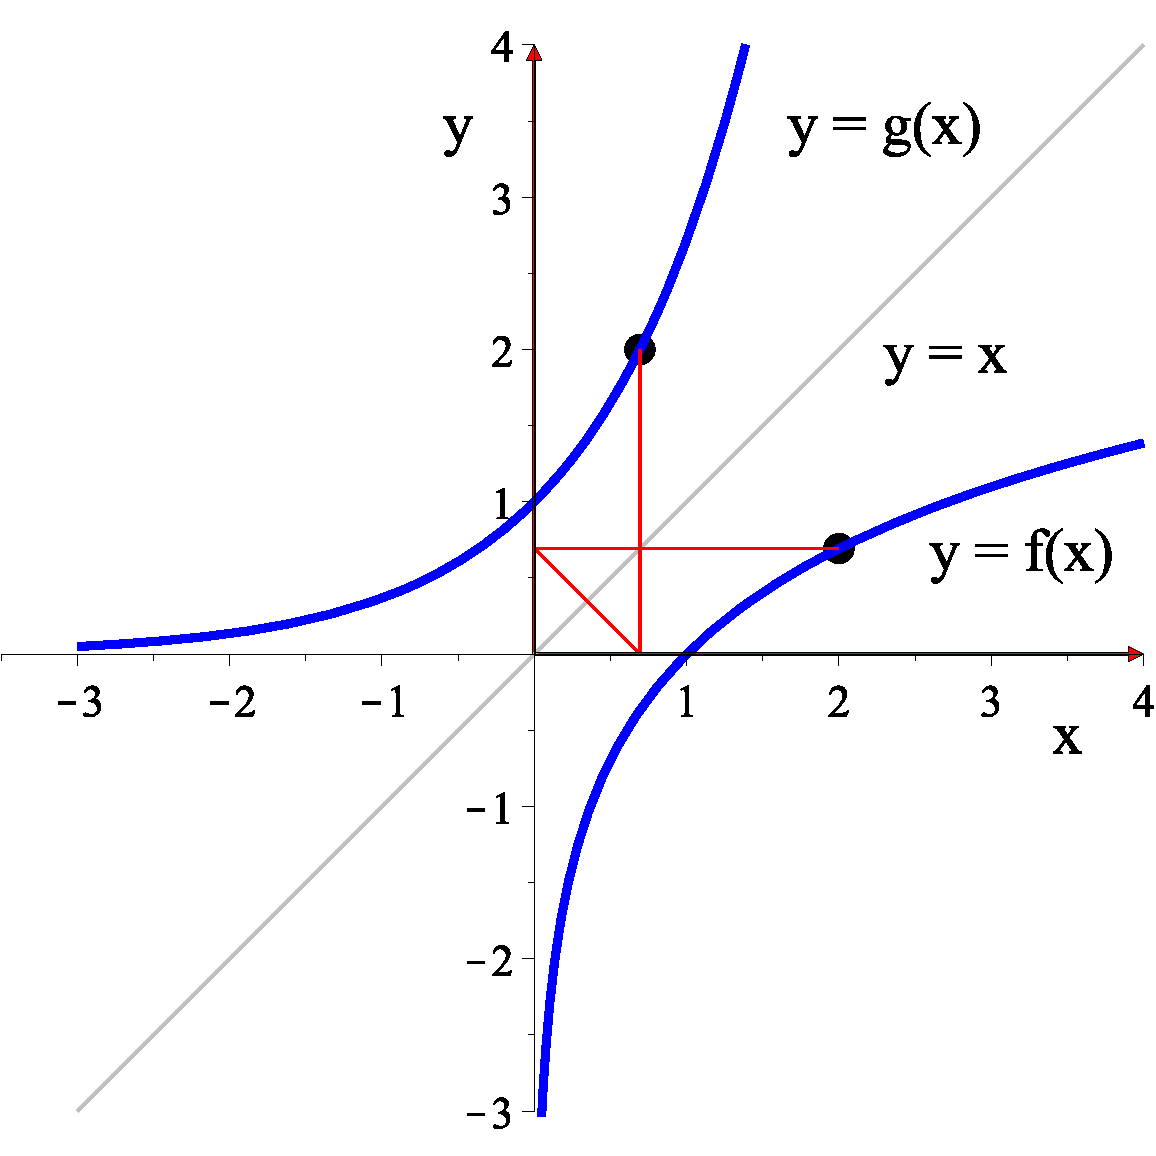
\includegraphics[height=120mm]{FIGS/plotOmvendt.pdf}}
\begin{center}
\caption{Grafen for en funktion $f(x)$ og grafen for dens omvendte funktion $g(x)$. Der gælder $g(x) = f^{\circ-1}(x)$ og $f(x) = g^{\circ-1}(x)$, men de har hver deres egne definitionsintervaller.} \label{tn14.figOmvendt}
\end{center}
\end{figure}


%%%%%%%%%%%%%%%%%%%%%%%%%%%%%%%%%%%%%%%%%%%%%%%%%%%%%%%%%%%%%
%%%%%%%%%%%%%%%%%%%%%%%%%%%%%%%%%%%%%%%%%%%%%%%%%%%%%%%%%%%%%
%%%%%%%%%%%%%%%%%%%%%%%%%%%%%%%%%%%%%%%%%%%%%%%%%%%%%%%%%%%%%

\subsection{Differentiation af omvendte funktioner}

\begin{theorem}[Differentiation af omvendt funktion]
Hvis en differentiabel funktion $f(x)$ har den omvendte funktion $f^{\circ-1}(x)$ og hvis $f'(f^{\circ-1}(x_{0})) \neq 0$, så er den omvendte funktion $f^{\circ-1}(x)$ selv differentiabel i $x_{0}$:
\begin{equation}
(f^{\circ-1})'(x_{0}) = \frac{1}{f'(f^{\circ-1}(x_{0}))}
\end{equation}
\end{theorem}
\begin{bevis}
Pr. definition af omvendt funktion gælder, at
\begin{equation}
h(x) = f(f^{\circ-1}(x)) = x \quad,
\end{equation}
så $h'(x_{0}) = 1$, men vi har så også fra kædereglen i (\ref{tn14.eqChain}):
\begin{equation}
h'(x_{0}) = f'(f^{\circ-1}(x_{0}))\cdot (f^{\circ-1})'(x_{0}) = 1 \quad ,
\end{equation}
hvoraf vi får resultatet ved at dividere med $f'(f^{\circ-1}(x_{0}))$.
\end{bevis}




%%%%%%%%%%%%%%%%%%%%%%%%%%%%%%%%%%%%%%%%%%%%%%%%%%%
%%%%%%%%%%%%%%%%%%%%%%%%%%%%%%%%%%%%%%%%%%%%%%%%%%%
%%%%%%%%%%%%%%%%%%%%%%%%%%%%%%%%%%%%%%%%%%%%%%%%%%%

\section{Hyperbolske funktioner}

\begin{definition}[Hyperbolsk cosinus og hyperbolsk sinus] \label{tn14.defCoshSinh}
Vi vil definere to nye funktioner $\cosh(x)$ og $\sinh(x)$ som de entydigt bestemte løsninger til følgende
differentialligningssystem med begyndelsesbetingelser. De to funktioner benævnes henholdsvis \ind{hyperbolsk cosinus}{hyperbolsk cosinus} og \ind{hyperbolsk sinus}{hyperbolsk sinus}:
\begin{equation} \label{tn14.eqCoshSinhDES}
\begin{aligned}
\cosh'(x) &= \sinh(x) \quad , \quad \cosh(0) = 1 \\
\sinh'(x) &= \cosh(x) \quad , \quad \sinh(0) = 0 \quad .
\end{aligned}
\end{equation}
\end{definition}

\emph{Betegnelserne} $\cosh(x)$ og $\sinh(x)$ ligner $\cos(x)$ og $\sin(x)$,
men funktionerne er meget forskellige, som vi skal se nedenfor.\\

Der er dog også fundamentale strukturelle ligheder mellem de to par af funktioner og det er dem der motiverer betegnelserne.
I differentialligningssystemet for $\cos(x)$ og $\sin(x)$ optræder kun et enkelt
minus-tegn som eneste forskel i forhold til (\ref{tn14.eqCoshSinhDES}):

\begin{equation}
\begin{aligned}
\cos'(x) &= -\sin(x) \quad , \quad \cos(0) = 1 \\
\sin'(x) &= \cos(x) \quad , \quad \sin(0) = 0 \quad .
\end{aligned}
\end{equation}

Desuden gælder (igen med et helt afgørende minustegn som eneste forskel) følgende  simple
analogi til den velkendte og ofte brugte relation $\cos^{2}(x) + \sin^{2}(x) = 1$:

\begin{theorem}[Fundamentale relation for $\cosh(x)$ og $\sinh(x)$]
\begin{equation} \label{tn14.eqFundamCoshSinh}
\cosh^{2}(x) - \sinh^{2}(x) = 1 \quad.
\end{equation}
\end{theorem}
\begin{bevis}
Differentier med hensyn til $x$ på begge sider af ligningen (\ref{tn14.eqFundamCoshSinh}) og konklud\'{e}r, at $\cosh^{2}(x) - \sinh^{2}(x)$ er en konstant. Brug
til sidst begyndelsesbetingelserne.
\end{bevis}

\begin{figure}[h]
\centerline{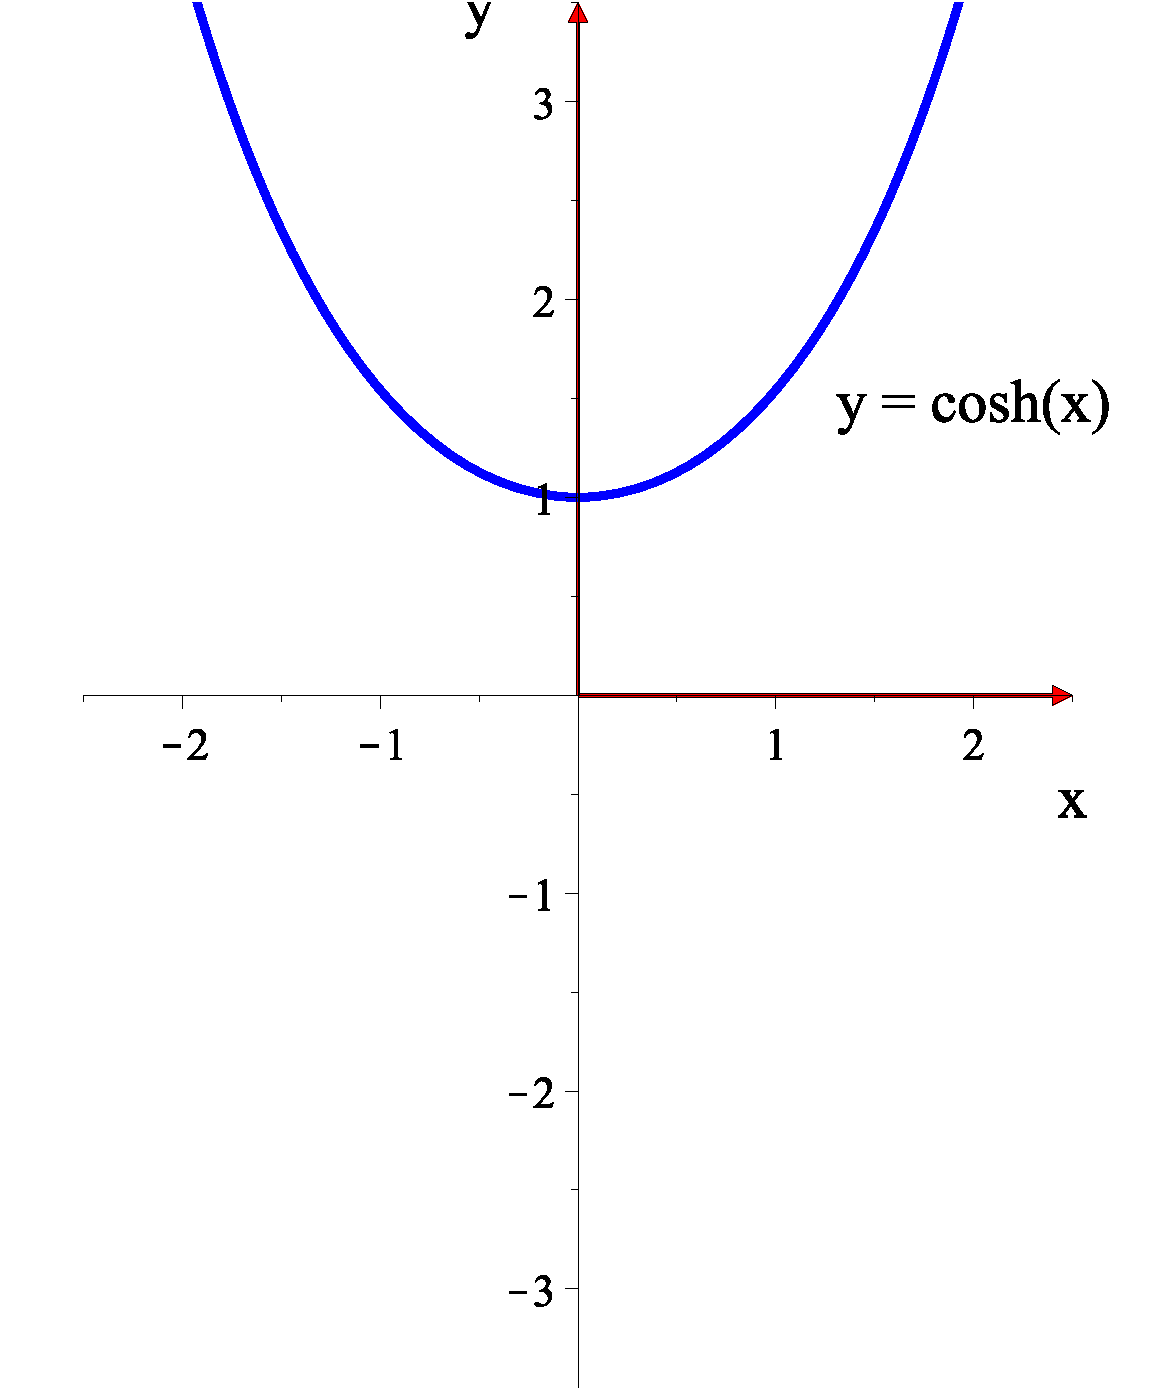
\includegraphics[width=65mm]{FIGS/plotcosh.pdf} \qquad 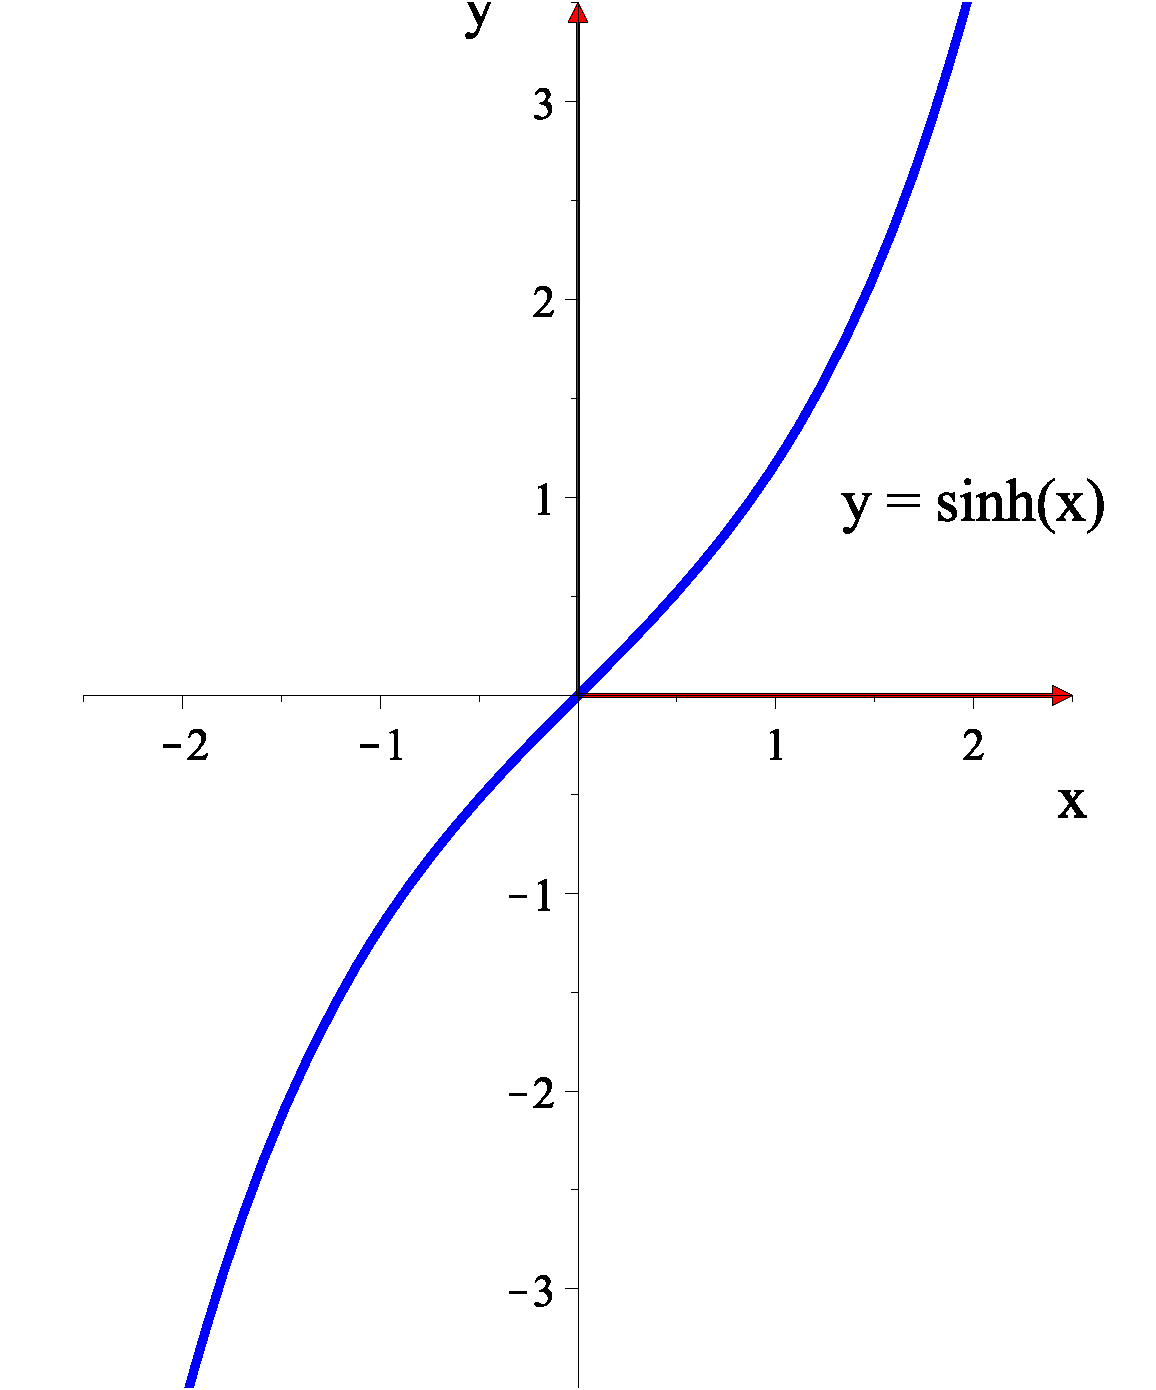
\includegraphics[width=65mm]{FIGS/plotsinh.pdf}}
\begin{center}
\caption{Hyperbolsk cosinus, $\cosh(x)$, og hyperbolsk sinus, $\sinh(x)$.} \label{tn14.figplotCoshSinh}
\end{center}
\end{figure}


\begin{exercise} \label{tn14.exercExplicCoshSinh}
Vis direkte ud fra differentialligningssystemet (\ref{tn14.eqCoshSinhDES}) at de to ''nye'' funktioner faktisk ikke er så nye endda:
\begin{equation}
\begin{aligned}
\cosh(x) &= \frac{e^x + e^{-x}}{2}\quad , \quad \mathcal{D}m(\cosh) = \mathbb{R}\quad , \quad \quad \mathcal{V}m(\cosh) = \,  [1, \infty[ \\
\sinh(x) &= \frac{e^x - e^{-x}}{2}\quad , \quad \mathcal{D}m(\sinh) = \mathbb{R}\quad , \quad \quad \mathcal{V}m(\sinh) = \, ]-\infty, \infty[
\end{aligned}
\end{equation}
\end{exercise}

\begin{exercise}
Vis \emph{direkte} ud fra de fundne udtryk i opgave \ref{tn14.exercExplicCoshSinh}, at
\begin{equation}
\cosh^{2}(x) - \sinh^{2}(x) = 1 \quad.
\end{equation}
\end{exercise}


\begin{exercise}
Grafen for funktionen $f(x) = \cosh(x)$ ligner meget en parabel, nemlig grafen for funktionen $g(x)= 1+ (x^{2}/2)$ når vi plotter begge funktionerne
i et passende lille interval omkring $x_{0}= 0$. Prøv det! Hvis vi derimod plotter begge graferne over et meget stort $x$-interval, vil vi opdage, at de to funktioner har meget forskellige grafiske opførsler. Prøv det, dvs. prøv at plotte begge funktioner over intervallet $[-50, 50]$.  Komment\'{e}r og forklar de kvalitative forskelle. Prøv tilsvarende at sammenligne de to funktioner $\sinh(x)$ og $x + (x^{3}/6)$ på samme måde.
\end{exercise}


Det er naturligt og nyttigt at definere de hyperbolske analogier til $\tan(x)$ og $\cot(x)$. Det gør vi således:

\begin{definition}[Hyperbolsk tangens og hyperbolsk cotangens]
\begin{equation}
\begin{aligned}
\tanh(x) &= \frac{\sinh(x)}{\cosh(x)} = \frac{e^{2x} -1}{e^{2x} + 1} \,\, , \,\, \mathcal{D}m(\tanh) = \mathbb{R}\,\,  , \,\,   \mathcal{V}m(\tanh) = \,  ]-1,1[ \\ \\
\coth(x) &= \frac{\cosh(x)}{\sinh(x)} = \frac{e^{2x}+1}{e^{2x} - 1} \,\, , \,\,
\mathcal{D}m(\coth) = \mathbb{R} - \{0\}\, \, , \\ &\phantom{\mathcal{D}m(\coth) = \mathbb{R} \setminus \{0\}\qquad \qquad} \mathcal{V}m(\coth) = \,  ]-\infty, -1[\, \cup\, ]1, \infty[ \quad .
\end{aligned}
\end{equation}
\end{definition}


\begin{figure}[h]
\centerline{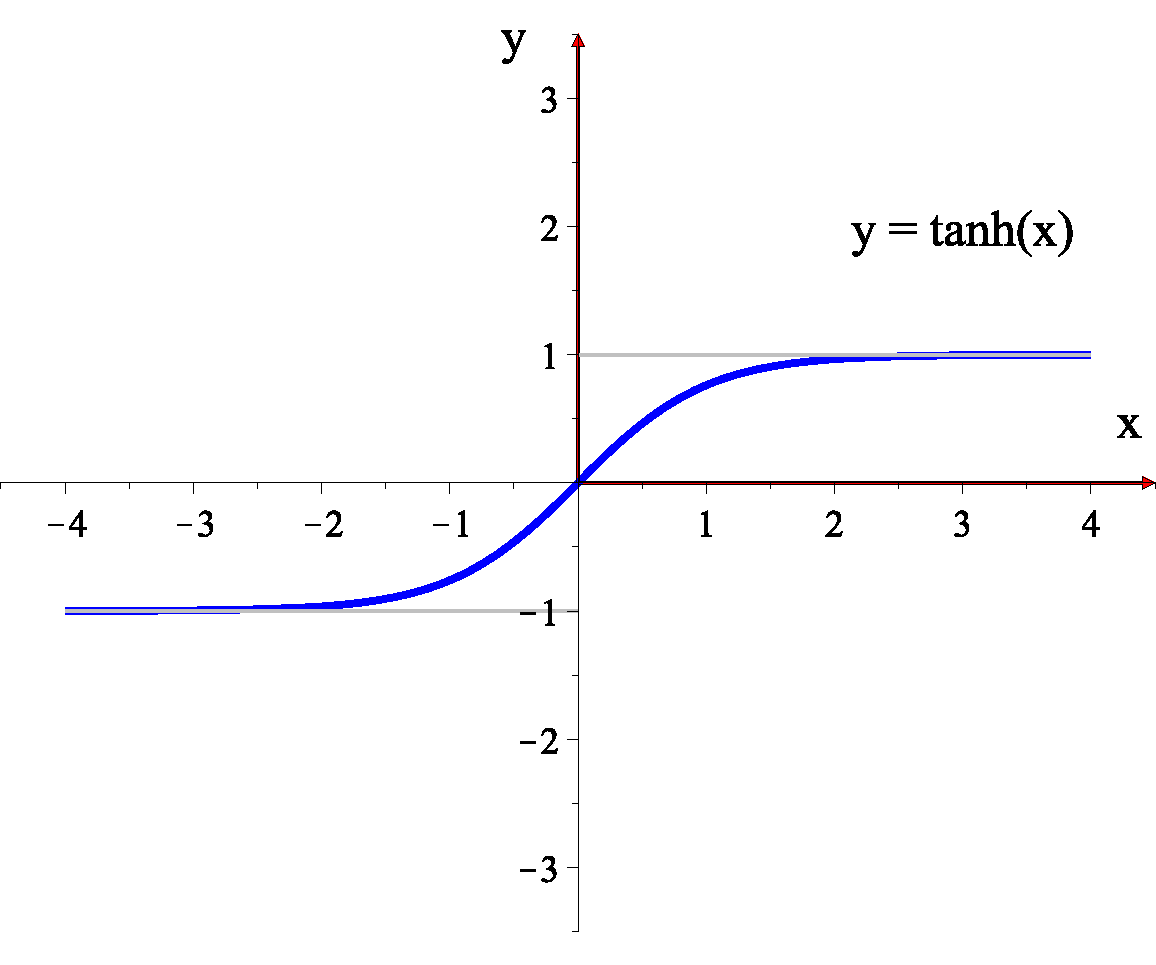
\includegraphics[width=75mm]{FIGS/plottanh.pdf} \quad \quad 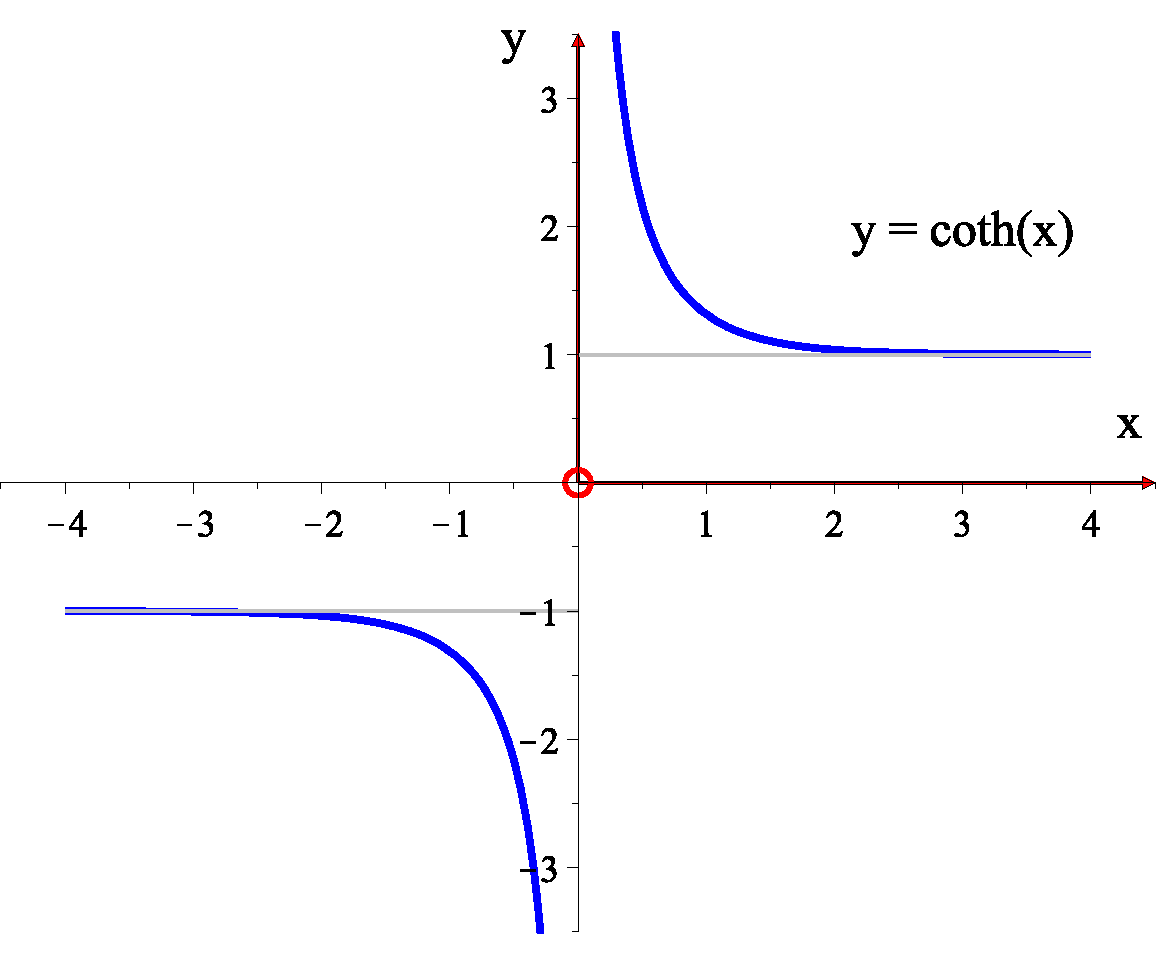
\includegraphics[width=75mm]{FIGS/plotcoth.pdf}}
\begin{center}
\caption{Hyperbolsk tangens, $\tanh(x)$, og hyperbolsk cotangens, $\coth(x)$.} \label{tn14.figplotTanhCoth}
\end{center}
\end{figure}




Differentialkvotienterne af $\cosh(x)$ og $\sinh(x)$ er allerede givet ved det definerende
system i (\ref{tn14.eqCoshSinhDES}).

\begin{equation} \label{tn14.eqHypDif}
\begin{aligned}
\frac{d}{dx}\cosh(x) &= \sinh(x) \\
\frac{d}{dx}\sinh(x) &= \cosh(x) \\
\frac{d}{dx}\tanh(x) &= \frac{1}{\cosh^{2}(x)} = 1 - \tanh^{2}(x) \\
\frac{d}{dx}\cosh(x) &= \frac{-1}{\sinh^{2}(x)} = 1 - \coth^{2}(x) \quad .
\end{aligned}
\end{equation}

\begin{exercise}
Vis de to sidste udtryk for differentialkvotienterne for $\tanh(x)$ og $\coth(x)$ i (\ref{tn14.eqHypDif}) ved at benytte differentiationsreglen i sætning \ref{tn14.thmFracDif}.
\end{exercise}

%%%%%%%%%%%%%%%%%%%%%%%%%%%%%%%%%%%%%%%%%%%%%%%%%%%
%%%%%%%%%%%%%%%%%%%%%%%%%%%%%%%%%%%%%%%%%%%%%%%%%%%

\section{Areafunktionerne}

De omvendte funktioner til de hyperbolske funktioner kaldes \ind{areafunktioner}{areafunktioner} og betegnes med henholdsvis
$\cosh^{\circ-1}(x) = \textrm{arcosh}(x)$, $\sinh^{\circ-1}(x) = \textrm{arsinh}(x)$, $\tanh^{\circ-1}(x) = \textrm{artanh}(x)$, og
$\coth^{\circ-1}(x) = \textrm{arcoth}(x)$.\\


Da funktionerne $\cosh(x)$, $\sinh(x)$, $\tanh(x)$, og $\coth(x)$ alle kan udtrykkes ved eksponentialfunktioner er det ikke overraskende, at de omvendte funktioner og deres differentialkvotienter kan udtrykkes ved logaritmefunktioner. Vi samler informationerne her:

\begin{equation}
\begin{aligned}
\textrm{arcosh}(x) &= \ln(x + \sqrt{x^{2} -1}) \, \, \textrm{for} \quad x \in [1, \infty[ \\
\textrm{arsinh}(x) &= \ln(x + \sqrt{x^{2} +1}) \, \, \textrm{for} \quad x \in \mathbb{R} \\
\textrm{artanh}(x) &= \frac{1}{2}\ln\left( \frac{1+x}{1-x}\right) \, \, \textrm{for} \quad x \in \, ]-1, 1[ \\
\textrm{arcoth}(x) &=\frac{1}{2}\ln\left( \frac{x-1}{x+1}\right) \, \, \textrm{for} \quad x \in \, ]-\infty , 1[ \,\cup \, ]1, \infty[ \quad .
\end{aligned}
\end{equation}
\begin{equation}
\begin{aligned}
\frac{d}{dx}\textrm{arcosh}(x) &=  \frac{1}{\sqrt{x^{2}-1}}   \, \, \textrm{for} \quad x \in ]1, \infty[ \\
\frac{d}{dx}\textrm{arsinh}(x) &=  \frac{1}{\sqrt{x^{2}+1}}   \, \, \textrm{for} \quad x \in \mathbb{R} \\
\frac{d}{dx}\textrm{artanh}(x) &=  \frac{1}{1 - x^{2}}   \, \, \textrm{for} \quad x \in  \, ]-1, 1[ \\
\frac{d}{dx}\textrm{arcoth}(x) &=  \frac{1}{1 - x^{2}}   \, \, \textrm{for} \quad x \in  \, ]-\infty\, 1[ \,\cup \, ]1, \infty[  \quad .
\end{aligned}
\end{equation}


%%%%%%%%%%%%%%%%%%%%%%%%%%%%%%%%%%%%%%%%%%%%%%%%%%%
%%%%%%%%%%%%%%%%%%%%%%%%%%%%%%%%%%%%%%%%%%%%%%%%%%%

\section{Arcusfunktionerne} \label{tn14.secArcus}

\begin{figure}[h]
\centerline{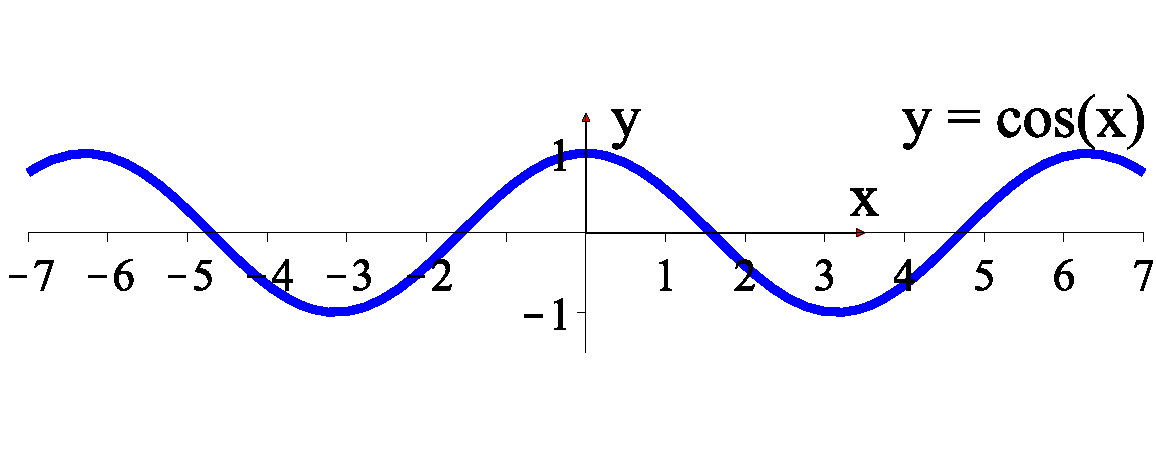
\includegraphics[width=80mm]{FIGS/plotcos.pdf} \quad 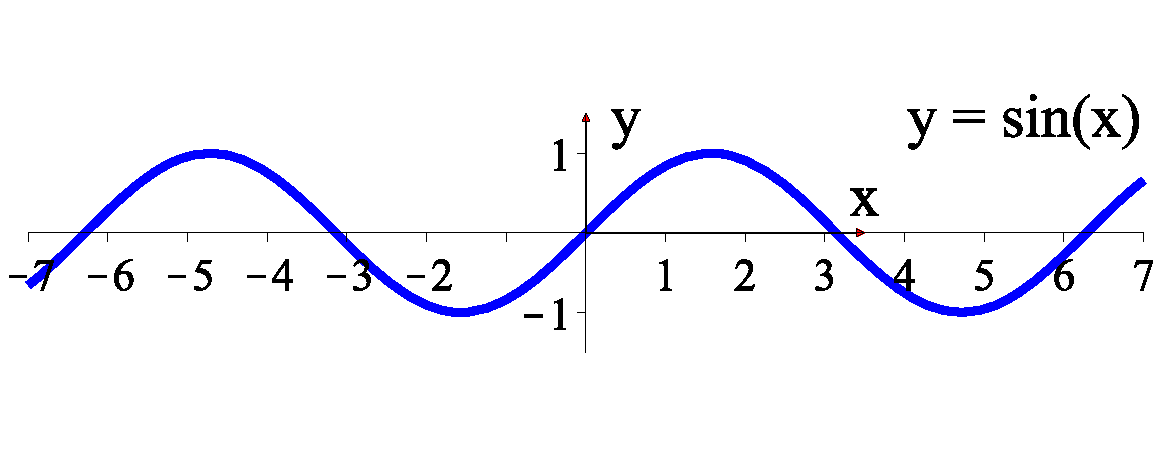
\includegraphics[width=80mm]{FIGS/plotsin.pdf}}
\begin{center}
\caption{Cosinus og sinus funktionerne.} \label{tn14.figplotcossin}
\end{center}
\end{figure}


De omvendte funktioner som hører til de trigonometriske funktioner er lidt mere komplicerede. Som nævnt bliver vi her nødt til for hver trigonometrisk funktion at vælge et interval, hvor den pågældende funktion er monoton. Til gengæld, når vi \emph{har} valgt et sådant interval, så er det klart, hvordan den omvendte funktion skal defineres og derefter hvordan den skal differentieres. De omvendte funktioner til $\cos(x)$, $\sin(x)$, $\tan(x)$, $\cot(x)$ betegnes henholdsvis $\arccos(x)$, $\arcsin(x)$, $\arctan(x)$, og $\textrm{arccot}(x)$; de benævnes arcus-cosinus, arcus-sinus, arcus-tangens, og arcuscotangens. Ligesom ovenfor samler vi resultaterne her:

\begin{equation}
\begin{aligned}
\cos^{\circ-1}(x) &= \arccos(x)  \in [0, \pi] \, \, \textrm{for} \quad x \in [-1, 1] \\
\sin^{\circ-1}(x) &= \arcsin(x)  \in [-\pi/2, \pi/2] \, \, \textrm{for} \quad x \in [-1, 1] \\
\tan^{\circ-1}(x) &= \arctan(x) \in [-\pi/2, \pi/2] \, \, \textrm{for} \quad x \in \mathbb{R} \\
\cot^{\circ-1}(x) &= \textrm{arccot}(x) \in ]0, \pi[ \, \, \textrm{for} \quad x \in \mathbb{R} \quad .
\end{aligned}
\end{equation}
\begin{equation}
\begin{aligned}
\frac{d}{dx}\arccos(x) &= \frac{-1}{\sqrt{1 - x^{2}}}\, \, \textrm{for} \quad x \in ]-1, 1[ \\
\frac{d}{dx}\arcsin(x) &= \frac{1}{\sqrt{1 - x^{2}}}\, \, \textrm{for} \quad x \in ]-1, 1[ \\
\frac{d}{dx}\arctan(x) &= \frac{1}{1+x^{2}}\, \, \textrm{for} \quad x \in \mathbb{R}\\
\frac{d}{dx}\textrm{arccot}(x) &= \frac{-1}{1+x^{2}} \, \, \textrm{for} \quad x \in \mathbb{R} \quad .
\end{aligned}
\end{equation}


\begin{figure}[h]
\centerline{\includegraphics[width=100mm]{FIGS/plotArccosSet.pdf}}
\begin{center}
\caption{Arcus-cosinus funktionen defineres her.} \label{tn14.figplotArccosSet}
\end{center}
\end{figure}


\begin{figure}[h]
\centerline{\includegraphics[width=65mm]{FIGS/plotArccos.pdf} \quad \quad  \includegraphics[width=65mm]{FIGS/plotArcsin.pdf}}
\begin{center}
\caption{Arcus-cosinus og arcus-sinus. De røde cirkler indikerer igen, at arcus-funktionerne ikke er defineret udenfor intervallet $[-1, 1]$. De grønne cirkelskiver indikerer tilsvarende, at arcus-funktionerne \emph{er} defineret i endepunkterne $x=1$ og $x=-1$.} \label{tn14.figplotArccossin}
\end{center}
\end{figure}



\begin{aha}
Læg mærke til, at differerentialkvotienterne for $\arccos(x)$ og $\arcsin(x)$ ikke er defineret i $x_{0}=1$ og i $x_{0}=-1$. Det skyldes dels, at hvis den funktion vi betragter kun er defineret i et begrænset interval, så kan vi ikke sige at funktionen er differentiabel i endepunkterne af intervallet. Desuden viser formlerne for  $\arccos'(x)$ og $\arcsin'(x)$ at de ikke er definerede i  $x_{0}= 1$ eller $x_{0}= -1$; de værdier giver jo $0$ i nævnerne.
\end{aha}


\begin{exercise}
Benyt en passende modifikation af $\arctan(x)$ til at konstruere en ny differentiabel (og derfor kontinuert) funktion $f(x)$, som ligner $0$-udvidelsen af $|x|/x$ (der hverken er kontinuert eller differentiabel), dvs. vi ønsker en funktion $f(x)$ med følgende egenskaber: $1> f(x) > 0.999$ for $x > 0.001$ og $-0.999 > f(x) > -1$ for $x < -0.001$. Se figur \ref{tn14.figplotArctan}.
Vink: Prøv at plotte $\arctan(1000x)$.
\end{exercise}


\begin{figure}[h]
\centerline{\includegraphics[width=120mm]{FIGS/plotArctan.pdf} }
\begin{center}
\caption{Arcus-tangens funktionen.} \label{tn14.figplotArctan}
\end{center}
\end{figure}


%%%%%%%%%%%%%%%%%%%%%%%%%%%%%%%%%%%%%%%%%%%%%%%%%%%
%%%%%%%%%%%%%%%%%%%%%%%%%%%%%%%%%%%%%%%%%%%%%%%%%%%
%%%%%%%%%%%%%%%%%%%%%%%%%%%%%%%%%%%%%%%%%%%%%%%%%%%
%%%%%%%%%%%%%%%%%%%%%%%%%%%%%%%%%%%%%%%%%%%%%%%%%%%



\begin{summary}
Vi har behandlet nogle af de fundamentale egenskaber ved nogle kendte og knap så kendte
funktioner. Hvordan er de defineret, hvad er deres definitions-intervaller, er de kontinuerte, er de differentiable, hvad
er i så fald deres differentialkvotienter?

\begin{itemize}
\item En funktion  $f(x)$ er kontinuert i $x_{0}$ hvis $f(x) - f(x_{0})$ er en epsilon-funktion af $(x - x_{0})$, dvs.
\begin{equation}
f(x) = f(x_{0}) + \varepsilon_{f}(x - x_{0}) \quad.
\end{equation}
\item En funktion $f(x)$ er differentiabel i $x_{0}$ med differentialkvotienten $f'(x_{0})$ hvis
\begin{equation*}
f(x) = f(x_{0}) + f'(x_{0})(x-x_{0}) + (x-x_{0})\varepsilon_{f}(x-x_{0})\quad .
\end{equation*}
\item Hvis en funktion er differentiabel i $x_{0}$, så er den også kontinuert i $x_{0}$. Det omvendte gælder \emph{ikke}.
\item Differentialkvotienten af et produkt af to funktioner er
\begin{equation}
\frac{d}{dx}\left(f(x)\cdot g(x)\right) = f'(x)\cdot g(x) + f(x)\cdot g'(x) \quad .
\end{equation}
\item Differentialkvotienten af en brøk mellem to funktioner er
\begin{equation}
\frac{d}{dx}\left( \frac{f(x)}{g(x)}\right) = \frac{f'(x)}{g(x)} - \frac{f(x) \cdot g'(x)}{g^{2}(x)}= \frac{f'(x)\cdot g(x) - f(x)\cdot g'(x)}{g^{2}(x)} \quad .
\end{equation}
\item Differentialkvotienten af en sammensat funktion er
\begin{equation} 
\frac{d}{dx} f(g(x)) = f'(g(x))\cdot g'(x) \quad .
\end{equation}

\item Differentialkvotienten af den omvendte funktion $f^{\circ-1}(x)$  er
\begin{equation}
\left(f^{\circ-1}\right)'(x) = \frac{1}{f'(f^{\circ-1}(x))} \quad .
\end{equation}
\end{itemize}



\end{summary}







%%%%%%%%%%%%%%%%%%%%%%%%%%%%%%%%%%%%%%%%%%%%%
%%%%%%%%%%%%%%%%%%%%%%%%%%%%%%%%%%%%%%%%%%%%%
%%% HER SKAL DU STOPPE MED AT SKRIVE %%%%%%%%
%%%%%%%%%%%%%%%%%%%%%%%%%%%%%%%%%%%%%%%%%%%%%
%%%%%%%%%%%%%%%%%%%%%%%%%%%%%%%%%%%%%%%%%%%%%


\end{document} 

%%%%%%%%%%%%%%%%%%%%%%%%%%%%%%%%%%%%%%%%%%%%%%%%%%%
%%%%%%%%%%%%%%%%%%%%%%%%%%%%%%%%%%%%%%%%%%%%%%%%%%% 